
\documentclass[letterpaper, 10 pt, conference]{ieeeconf}
\IEEEoverridecommandlockouts
\usepackage{graphicx}
\usepackage{amsmath}
\usepackage{amssymb}
\usepackage{amsfonts}
\usepackage{booktabs}
\usepackage{xcolor}
\usepackage{url}
\usepackage{algorithm}
\usepackage{algpseudocode}
% A figure* placed right after \maketitle silently defers to page 2 in this
% class, because \maketitle zeroes the top-of-page float counters as part of
% its own \twocolumn[...] title block. The class's documented escape hatch is
% \IEEEaftertitletext{}: content injected there renders as part of the
% guaranteed single-column title block itself, not as a float, so it cannot be
% deferred. capt-of then gives it a normal numbered "Fig. 1" caption outside a
% float environment.
\usepackage{capt-of}


%%%%%%%%%%%%%%%%%%%%%%%%%%%%%%%%%%%%%%%%%%%%%%%%%%%%
\title{\LARGE \bf
Constraint-Aware Pick-Throw-Place:
Data-Efficient Model-Based Learning of Whole-Trajectory Feasible
Release States for Low-Torque Manipulators
}
\author{Anonymous submission}

%\author{ Dharmendra Sharma, Rohit Jangra, Deepak Raina, Narendra Kumar Dhar}
%\IEEEauthorblockA{Indian Institute of Technology Mandi, India}

\begin{document}

\maketitle

%%%%%%%%%%%%%%%%%%%%%%%%%%%%%%%%%%%%%%%%%%%%%%%%%%%%%%%%%%%%%%%%%%%%%%%%%%%%%%%%
\begin{abstract}
Pick-throw-place (PTP) can extend a robot's effective workspace for applications such as sorting and material handling: an object released with a controlled velocity follows a ballistic trajectory during free flight and can be deposited beyond the arm's reach. Accurate throwing is difficult for manipulators with limited torque and velocity capabilities, and becomes harder still when aerodynamic drag on the object is not negligible. Recent model-based reinforcement learning (MBRL) approaches enable data-efficient throwing from few physical trials. However, these approaches typically rely on a predefined release configuration that may become infeasible when transferred to manipulators with lower torque and velocity limits. We address this limitation by introducing a constraint-aware release-state search that selects the release posture, direction, and achievable release speed according to arm-specific limits (joint position, joint velocity, and actuator torque). Candidate release states are further evaluated over the complete windup, throw, and post-release follow-through trajectories, rather than only at the release instant. The resulting release-state table is integrated with a sparse Gaussian-process dynamics model and particle-based policy optimization to learn target-dependent release speeds. Across four robotic manipulators in rigid-body simulation--KUKA iiwa7, Franka Panda, xArm6, and Kinova Gen3--the learning pipeline yields $1.4$--$2.7$~cm mean landing error without arm-specific policy tuning, and the release-state search transfers to a 6-DOF UR7e without algorithmic change. A single target-conditioned policy transfers over a continuous range of target heights ($0$--$0.45$~m), giving $2.13$~cm mean error at heights never seen during training. A drag sweep places the crossover at which learning starts to pay: below $1\%$ drag the no-drag analytical baseline is the more accurate model, and at $19\%$ it is $4.3$--$4.6\times$ worse. Finally, hardware experiments on the Kinova Gen3 execute the full stack with an object in the gripper and quantify the release-timing terms that govern transfer: a command lag that shortens the throw, a late object departure that lengthens it, and the instant at which they cancel.
\end{abstract}

\begin{keywords}
Pick-throw-place, model-based reinforcement learning, Gaussian process regression, constraint-aware motion planning, and dynamic manipulation
\end{keywords}
%%%%%%%%%%%%%%%%%%%%%%%%%%
%%%%%%%%%%%%%%%%%%%%%%%%%

\section{Introduction}
\label{sec:intro}

\begin{figure}[t]
    \centering
    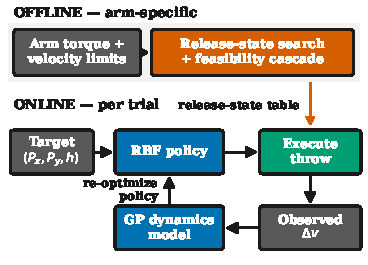
\includegraphics[width=0.45\textwidth]{figs/fig_pipeline.pdf}
    \caption{Overview of the proposed constraint-aware model-based
    PTP framework. The offline stage is executed once per
    manipulator; the online stage repeats once per training trial.}
    \label{fig:pipeline}
\end{figure}

Pick-throw-place (PTP) provides an efficient alternative to conventional pick-and-place for applications such as sorting and material handling. By releasing an object with a controlled velocity and letting it follow a ballistic trajectory during free flight, a manipulator can deposit objects beyond its conventional end-effector workspace and reduce the transport motion required for each cycle. However, accurate throwing requires a fast and precisely timed release that remains within the manipulator's kinematic and dynamic limits (joint position, joint velocity, and actuator torque). Small errors in release position, velocity, or timing can result in substantial landing errors, while limited actuator torque and joint velocity can prevent the arm from generating a useful release motion in the first place.

Recent model-based reinforcement learning (MBRL) methods have made robotic throwing substantially more data efficient. MC-PILOT~\cite{turcato2025mcpilot}, for example, combines sparse Gaussian-process (GP) dynamics learning with particle-based policy optimization to learn target-dependent release speeds from a small number of physical trials. Building on MC-PILCO~\cite{amadio2022mcpilco} and earlier model-based tossing work~\cite{turcato2023codit}, this formulation reduces the learning problem by prescribing a release configuration and analytically generating the joint motion that reaches it. This decomposition is effective on the 7-DOF Franka Emika Panda, but it assumes that the prescribed release configuration can be realized by the manipulator.

However, this assumption becomes restrictive when the same throwing strategy is transferred to a manipulator with lower actuator torque capacity. On the Kinova Gen3, whose wrist actuators provide substantially less torque than those of the Franka Emika Panda, directly adopting the fixed-release strategy does not produce a useful high-elevation throw. Under the predefined release posture, increasing the release elevation reduces the achievable range, causing distance-based optimization to favor a near-horizontal motion rather than a genuine throw. This observation indicates that the release configuration cannot be treated as a platform-independent design constant; instead, it must be selected according to the kinematic and dynamic capabilities of the specific manipulator.

Analytical formulations provide fast and interpretable solutions by deriving release conditions from ballistic and manipulator models. Lynch and Mason~\cite{lynch1999dynamic} established throwing, catching, and batting as forms of dynamic manipulation that exploit gravity and momentum. More recent work has characterized reachable tossing workspaces and learned release-velocity mappings for bimanual systems~\cite{bombile2023bimanual}. While these approaches provide useful geometric and dynamical insight, their performance depends on model fidelity and on the feasibility of the resulting motion.

Learning-based methods reduce dependence on an exact analytical model. TossingBot~\cite{zeng2020tossingbot} learns throwing directly from robot interaction using residual physics, while Monastirsky et al.~\cite{monastirsky2023learning} formulate throwing as sequence modeling to transfer simulation-trained behavior using limited physical data. Other approaches extend dynamic manipulation to bimanual handover~\cite{huang2023dynamic}, whole-body manipulation~\cite{munn2024wholebody}, and mobile-manipulator catching~\cite{zhang2025catch}. These methods demonstrate the effectiveness of learning for dynamic manipulation, but they do not directly address how to select a feasible release motion for a fixed-base, low-torque manipulator while retaining the data efficiency of model-based policy search.

A related line of work considers actuator and trajectory constraints explicitly. Manipulator trajectory optimization commonly incorporates joint-position, velocity, acceleration, and torque limits, which are particularly important for high-speed motions. Werner et al.~\cite{werner2024dynamic} exploit passive joints of an underactuated, torque-limited material-handling machine to generate dynamic throws beyond its static reach, while Liu et al.~\cite{liu2022adaptive} formulate planar throwing feasibility for online replanning under disturbance. Moura et al.~\cite{moura2022nonprehensile} demonstrate constraint-aware trajectory optimization for dynamic manipulation. These methods motivate considering feasibility throughout the motion; however, they do not combine arm-specific release-state selection with sparse-GP model-based throwing on a fixed-base, torque-limited manipulator.

Motivated by these limitations, we propose a constraint-aware model-based framework for data-efficient PTP on manipulators with limited kinematic and dynamic capabilities. Our key contributions are summarized as follows. First, we propose a novel arm-specific release-state search that determines the release posture, direction, and achievable release speed from the manipulator's own kinematic and dynamic limits, in place of a release configuration prescribed a priori. Second, we introduce a whole-trajectory feasibility cascade that evaluates the windup, release, and post-release follow-through motions rather than checking feasibility only at the release instant, enabling us to quantify its effect on the achievable throwing range. Third, we integrate the resulting release-state representation with sparse Gaussian-process dynamics learning and particle-based policy optimization to enable data-efficient target-dependent throwing, and investigate target-height generalization -- whether one policy conditioned on target height covers an interval of heights rather than a few discrete ones -- and the operating regimes in which model-based learning improves over a no-drag analytical model. Finally, we demonstrate that the formulation is not tied to one arm, and we bring the same release solver to a physical Kinova Gen3, validating the execution components it requires. An overview of the proposed offline and online pipeline is shown in Fig.~\ref{fig:pipeline}.


%%%%%%%%%%%%%%%%%%%%%%%%%%%%%%%%%%%%%%%%%%%%%%%%%%%%%%%%%%%
% \section{Constraint-Aware Model-Based Pick-Throw-Place}

% \subsection{Problem Formulation and Learning Framework}
% Following MC-PILOT~\cite{turcato2025mcpilot}, we formulate pick-and-throw as a
% model-based policy-search problem. A sparse GP model approximates the object's
% velocity dynamics from collected transitions, and particle-based policy
% optimization searches for a target-conditioned release speed. The main
% modification is that the release configuration is no longer fixed a priori;
% instead, we first determine a release state that is kinematically and
% dynamically feasible for the selected manipulator.

% The complete pipeline therefore has three stages. First, a robot-specific
% release-state search determines a feasible release posture, direction, and
% maximum achievable release speed. Second, the resulting release-state table is
% integrated with the GP-based policy optimization. Third, the learned policy is
% evaluated using a rigid-body simulation of the complete arm and object dynamics
% rather than the training-time particle cost alone. The same release solver is
% used for simulation and hardware execution. Algorithm~\ref{alg:pipeline}
% summarizes the offline search and the online model-based learning loop.

% Following~\cite{turcato2025mcpilot}, the object dynamics are represented by
% three independent sparse GPs, one per Cartesian velocity component. Each GP is
% trained on transitions of the form
% $(\text{position},\text{velocity})\rightarrow\Delta\text{velocity}$ collected
% from throwing trials. An RBF policy maps the target position---and, in the
% height-generalized formulation, the target height---to a release speed.

% The policy output is constrained to $[0,u_M]$ using
% \begin{equation}
% u=\frac{u_M}{2}\left(\tanh(x)+1\right),
% \label{eq:policy-squash}
% \end{equation}
% where $x$ is the unconstrained policy output. During policy optimization,
% particles are propagated through the learned GP dynamics and the policy is
% updated to minimize expected landing distance. Because optimization is
% performed against the learned model, policy improvement between physical trials
% requires no additional robot interaction.

% \begin{algorithm}[t]
% \caption{Constraint-Aware Model-Based Pick-Throw-Place}
% \label{alg:pipeline}
% \begin{algorithmic}[1]
% \Statex \textbf{Offline release-state search} \emph{(once per arm/workspace)}
% \State \textbf{input:} URDF; limits $\dot q^{\max},\tau_{\max}$; target range
% \State $\mathcal{C}\gets\emptyset$
% \For{each posture $q$ and static offset on the grid}
%     \If{EE height or static-gravity torque infeasible}
%         \State \textbf{continue}
%     \EndIf
%     \For{each direction $\hat d$ (elev.\ $5^\circ$--$45^\circ$, both signs)}
%         \State $s^\star\gets$ inner LP~\eqref{eq:release-lp} (max release speed)
%         \If{candidate passes cascade (Sec.~\ref{sec:method-feasibility})}
%             \State $R\gets$ landing distance (drag-augmented integration)
%             \State $\mathcal{C}\gets\mathcal{C}\cup\{(q,\dot q,\hat d,s^\star,R)\}$
%         \EndIf
%     \EndFor
% \EndFor
% \State $(q,\dot q)^{\mathrm{rel}}\!\gets\!\arg\max_{\mathcal{C}} R$;\ propagate over
% azimuth $\rightarrow$ table $\mathcal{T}$
% \Statex \textbf{Online model-based learning} \emph{(per trial)}
% \State collect exploration throws; fit sparse GP dynamics $\mathcal{G}$
% \For{trial $=1,\dots,N$}
%     \State optimize RBF policy $\pi$ against $\mathcal{G}$ (particle rollout)
%     \State execute: $\pi\!\rightarrow\! s$; look up $\mathcal{T}$; computed
%     torque~\eqref{eq:computed-torque}
%     \State measure release velocity and landing; update $\mathcal{G}$
% \EndFor
% \end{algorithmic}
% \end{algorithm}

% \subsection{Release-State Optimization}
% \label{sec:method-search}

% The original formulation fixes the release joint configuration
% $q_{\mathrm{rel}}$ and learns only the target-dependent release speed and
% aiming variables. We instead search over the release state $(q,\dot q)$. The
% search has two levels: an outer enumeration over candidate release postures and
% directions, and an inner optimization that determines the maximum release speed
% achievable at each candidate.

% \textbf{Inner release-speed optimization.}
% For the 7-DOF Gen3, the three pitch joints provide the dominant contribution to
% velocity perpendicular to the selected swing plane. The four roll/twist joints
% are therefore held at zero velocity during release-state optimization:
% \begin{equation}
% \begin{aligned}
% \max_{\dot q,\,s}\quad &s\\
% \text{s.t.}\quad &J(q)\dot q=s\,\hat d,\\
% &|\dot q_i|\leq\dot q_i^{\max},\qquad \forall i,\\
% &\dot q_i=0,\qquad i\in\{0,2,4,6\}.
% \end{aligned}
% \label{eq:release-lp}
% \end{equation}
% Here $s$ is the release speed and $\hat d$ is the desired unit release
% direction. The problem is linear in $(\dot q,s)$ and is solved with
% \texttt{scipy.optimize.linprog} using the HiGHS solver.

% The static angles of the roll/twist joints remain free search variables. They
% are not assigned velocities because letting them contribute to release motion
% can produce a rotational component poorly aligned with the desired throwing
% direction; a nonzero static offset also prevents the pitch axes from becoming
% geometrically degenerate.

% \textbf{Outer posture and direction search.}
% Candidate release postures are obtained by grid-searching the relevant joint
% angles and static offsets. For each posture, we first check the minimum
% end-effector height and static gravity-induced torque feasibility. Candidate
% release directions are then sampled within the posture-dependent swing plane,
% using elevation angles from $5^\circ$ to $45^\circ$ at $5^\circ$ increments and
% both elevation signs.

% For every surviving posture--direction pair, the inner optimization in
% Eq.~\eqref{eq:release-lp} determines the maximum feasible release speed.
% Candidates are then evaluated by the complete feasibility cascade of
% Sec.~\ref{sec:method-feasibility}. Among candidates that pass all checks, the
% release state that maximizes the true landing distance is selected. Landing
% distance is computed by forward integration of the drag-augmented ballistic
% dynamics from the candidate's actual release position and velocity.

% \subsection{Azimuth Propagation}

% Once verified for a given arm and workspace, the release state is propagated
% over the required base-azimuth range by rotating the base joint. Because
% gravity is invariant under rotation about the vertical axis, the Jacobian and
% feasibility properties rotate consistently with the base angle, so we construct
% an azimuth-to-pose table rather than independently optimizing every azimuth.

% For the Gen3, the verified release state is propagated over a $-33^\circ$ to
% $+33^\circ$ azimuth range at $3^\circ$ increments, and a turret-aiming
% correction accounts for the offset between the tabulated release geometry and
% the target bearing. The same \texttt{OptimizedReleaseSolver} is used during
% training and execution; a regression test asserts that the simulation and
% hardware planners agree to within $10^{-12}$ on the resulting release state.

% \subsection{Whole-Trajectory Feasibility}
% \label{sec:method-feasibility}

% Release-instant feasibility alone does not guarantee that the complete throwing
% motion can be executed within the manipulator's limits. We therefore evaluate
% each candidate using four sequential checks; a candidate is rejected at the
% first stage it fails.
% \begin{enumerate}
%     \item \textbf{Kinematic windup bound.} The windup configuration
%     \begin{equation}
%     q_{\mathrm{windup}}
%     =
%     q_{\mathrm{rel}}
%     -
%     \dot q_{\mathrm{rel}}\frac{t_{\mathrm{throw}}}{2}
%     \end{equation}
%     must satisfy all joint-position limits.

%     \item \textbf{Windup-path torque.} We sample the neutral-to-windup motion
%     and evaluate gravity-induced inverse dynamics at five intermediate
%     configurations. Torque must remain below $90\%$ of the corresponding
%     manufacturer limit.

%     \item \textbf{Throw-ramp torque.} The exact cubic windup-to-release
%     velocity profile used by the runtime controller is evaluated at 40 points.
%     In addition to inverse dynamics, the calculation includes the
%     Jacobian-transpose feedforward term associated with the gripped object's
%     weight. The resulting torque must remain below $75\%$ of the corresponding
%     limit.

%     \item \textbf{Follow-through torque and velocity.} The post-release
%     recovery motion is evaluated over eight candidate recovery durations from
%     $0.6$ to $4.0$~s, with 30 samples per duration. Both torque and
%     joint-velocity limits are checked; a candidate is accepted if at least one
%     recovery duration satisfies the specified margins.
% \end{enumerate}

% This cascade explicitly captures failure modes that are invisible to a
% release-state-only check: a candidate can satisfy torque constraints at release
% while violating them during the windup or while recovering from a high-speed
% release.

% \subsection{Dynamics-Aware Throw Execution}
% \label{sec:method-torque}

% To evaluate the release state through the arm and object dynamics, the
% simulated manipulator is controlled using computed torque:
% \begin{equation}
% \tau =
% M(q)\ddot q_{\mathrm{cmd}}
% +
% C(q,\dot q)
% +
% G(q)
% +
% J(q)^\top f_{\mathrm{ball}},
% \label{eq:computed-torque}
% \end{equation}
% where $M$, $C$, and $G$ are the manipulator mass, Coriolis/centrifugal, and
% gravity terms. The final term explicitly compensates for the weight of the
% gripped object,
% \begin{equation}
% f_{\mathrm{ball}}=m_{\mathrm{ball}}[0,0,g]^\top .
% \end{equation}
% The ball is modeled as a separate rigid body attached through a removable grip
% constraint, so the explicit feedforward term accounts for the payload even
% though it is not part of the manipulator's kinematic chain.

% The attachment point is offset from the wrist flange by the gripper's tool
% center point, $r_{\mathrm{offset}}=0.12$~m, applied consistently to the
% release-speed optimization (Eq.~\eqref{eq:release-lp}, with the Jacobian
% evaluated at the tool point) and to the simulation, where the ball is welded at
% the same point. Because the wrist is rotating at release, this offset
% contributes an additional velocity component $\omega\times r_{\mathrm{offset}}$
% that a flange-attached model omits---approximately $+0.39$~m/s ($+26\%$) and a
% $1.24^\circ$ direction change at the release state where this was measured.
% Placing the attachment point correctly reproduces this contribution directly
% from the rigid-body physics, without a manually derived correction term.

% Release velocity is measured from the physics engine after the grip constraint
% is removed rather than assigned directly, ensuring that the reported release
% velocity is the velocity actually produced by the simulated arm.

% Three further mismatches were fixed during validation: targets are sampled in
% flight space around the release point rather than the base origin (which had
% produced unreachable off-axis targets); the particle model uses the empirical
% mean release position from collected trials rather than the nominal one; and
% the windup trajectory is rendered and checked to rule out a zero-amplitude
% windup.

% \subsection{Height-Generalized Policy}

% To evaluate generalization beyond a single landing plane, both the
% trajectory-termination plane and the particle propagation are parameterized by
% the target height $h$, so the policy input becomes $(P_x,P_y,h)$. We compare
% three settings: a policy trained at one fixed height; separate policy
% re-optimization for discrete target heights while reusing the learned GP; and a
% single policy trained over a continuous range of target heights. The third
% setting tests whether the learned model can support interpolation to target
% heights absent from the training data, without a separate policy-optimization
% run for each height.
%%%%%%%%%%%%Section_II_Proposed_work_%%%%%%%%%%

\section{Constraint-Aware Model-Based Pick-Throw-Place}
\label{sec:approach}

We formulate PTP as a model-based policy-search problem in which
object dynamics are learned from a small number of throwing trials and a
target-conditioned policy determines the release speed. Following
MC-PILOT~\cite{turcato2025mcpilot}, we use sparse Gaussian-process (GP)
dynamics and particle-based policy optimization. However, rather than fixing
the release configuration a priori, we first determine a release state that is
consistent with the kinematic and dynamic limits of the selected manipulator.

The resulting framework separates arm-specific feasibility computation from
data-efficient model learning. An offline search identifies feasible release
postures, directions, and release speeds and stores them in an azimuth-indexed
release-state table. Online, the policy selects the release speed for the
target, the corresponding release state is retrieved from the table, and
observed throwing transitions are used to update the GP model. As shown in
Fig.~\ref{fig:pipeline}, the offline release-state search depends only on the
manipulator's torque and velocity limits and is therefore executed once per
arm and workspace, whereas the policy, the executed throw, and the GP model
form a loop that repeats once per training trial. The complete procedure is
summarized in Algorithm~\ref{alg:pipeline}.

\subsection{Problem Formulation and Learning Framework}
\label{sec:method-formulation}

The object dynamics are represented by three independent sparse GPs, one for
each Cartesian velocity component. Each GP models the velocity increment
\begin{equation}
(\mathbf{p},\mathbf{v}) \rightarrow \Delta\mathbf{v},
\end{equation}
where $\mathbf{p}\in\mathbb{R}^{3}$ and $\mathbf{v}\in\mathbb{R}^{3}$ denote
the object position and velocity. The models are learned from transitions
collected during throwing trials and are subsequently used to propagate
particles during policy optimization. Each GP is sparse: rather than retaining
every collected transition, it is summarized by a fixed set of $M$ inducing
points and trained on mini-batches of $N_b$ transitions, which bounds both
memory and per-iteration cost as trials accumulate.

The policy is represented by a radial basis function (RBF) model that maps the
target state to a release speed. For the standard formulation, the target
position is used as input; for target-height generalization, the target height
is included as an additional input. The unconstrained policy output $x$ is
mapped to the feasible release-speed interval $[0,u_M]$ as
\begin{equation}
u=\frac{u_M}{2}\left(\tanh(x)+1\right),
\label{eq:policy-squash}
\end{equation}
where $u_M$ is the maximum release speed associated with the selected release
state.

During policy optimization, particles are propagated through the learned GP
dynamics and the policy parameters are optimized to minimize the expected
landing distance to the target. Since optimization is performed against the
learned model, the policy can be re-optimized between physical trials without
additional robot interaction. The release-state search therefore provides the
constraint-aware action space, while model-based learning determines the
target-dependent release speed within that space.

\begin{algorithm}[t]
\caption{Constraint-Aware Model-Based Pick-Throw-Place}
\label{alg:pipeline}
\begin{algorithmic}[1]
\Statex \textbf{Offline release-state search} \emph{(once per arm/workspace)}
\State \textbf{Input:} URDF; limits $\dot q^{\max},\tau_{\max}$; target range
\State $\mathcal{C}\gets\emptyset$
\For{each posture $q$ and static offset on the grid}
    \If{EE height or static-gravity torque infeasible}
        \State \textbf{continue}
    \EndIf
    \For{each direction $\hat d$ (elev.\ $5^\circ$--$45^\circ$, both signs)}
        \State $s^\star\gets$ inner LP~\eqref{eq:release-lp}
    \If{candidate passes feasibility cascade}
        \State $R\gets$ landing distance from drag-augmented integration
        \State $\mathcal{C}\gets
        \mathcal{C}\cup\{(q,\dot q,\hat d,s^\star,R)\}$
    \EndIf
    \EndFor
\EndFor
\State $(q,\dot q)^{\mathrm{rel}}\gets
\arg\max_{\mathcal{C}}R$; propagate over azimuth $\rightarrow\mathcal{T}$
\Statex \textbf{Online model-based learning}
\State collect exploration throws; fit sparse GP dynamics $\mathcal{G}$
\For{trial $=1,\ldots,N$}
    \State optimize RBF policy $\pi$ against $\mathcal{G}$ using particle rollout
    \State execute $\pi\rightarrow s$; retrieve release state from $\mathcal{T}$
    \State execute computed-torque trajectory~\eqref{eq:computed-torque}
    \State measure release velocity and landing outcome; update $\mathcal{G}$
\EndFor
\end{algorithmic}
\end{algorithm}

\subsection{Release-State Search}
\label{sec:method-search}

The release state is defined by the joint configuration and velocity
$q,\dot q\in\mathbb{R}^{n}$, with $\tau_{\max}$ and $\dot q^{\max}$ denoting the
corresponding manufacturer actuator limits ($n=7$ for the manipulators
considered here). Rather than fixing $q_{\mathrm{rel}}$, we search over candidate
postures and release directions and determine the maximum feasible release
speed for each candidate. This search separates geometric selection from the
velocity optimization required to realize a specified release direction.

For the 7-DOF Kinova Gen3, the three pitch joints provide the dominant
contribution to the end-effector velocity in the selected swing plane. The four
roll/twist joints are therefore assigned zero release velocity, yielding the
linear program
\begin{equation}
\begin{aligned}
\max_{\dot q,\,s}\quad &s\\
\text{s.t.}\quad
&J(q)\dot q=s\,\hat d,\\
&|\dot q_i|\leq\dot q_i^{\max},\qquad \forall i,\\
&\dot q_i=0,\qquad i\in\{0,2,4,6\}.
\end{aligned}
\label{eq:release-lp}
\end{equation}
Here, $s$ is the release speed, $\hat d$ is the desired unit release direction,
and $J(q)$ is the manipulator Jacobian obtained by forward kinematics at the
release configuration. The problem is linear in the decision variables
$(\dot q,s)$, so its global optimum is obtained directly by linear programming
and no initial guess or local search is required.

The static angles of the roll/twist joints remain free search variables. Their
release velocities are set to zero to avoid introducing motion components that
are poorly aligned with the desired throwing direction, while their static
offsets also prevent geometric degeneracy of the pitch-joint swing mechanism.

Candidate postures are generated by grid-searching the relevant joint angles
and static offsets. Each posture is first checked by forward kinematics for the
required end-effector height, and by inverse dynamics for the static
gravity-induced torque it demands. For feasible postures,
release directions are sampled within the corresponding swing plane using
elevation angles from $5^\circ$ to $45^\circ$ in $5^\circ$ increments and both
elevation signs. The inner optimization in Eq.~\eqref{eq:release-lp} then
provides the maximum release speed for each posture--direction pair.

The resulting candidates are evaluated using the complete trajectory
feasibility cascade described in Sec.~\ref{sec:method-feasibility}. Among the
candidates that satisfy all constraints, the release state maximizing the
predicted landing distance is selected. The landing distance is obtained by
forward integration of the drag-augmented ballistic dynamics using the
candidate's actual release position and velocity.

Once the release state has been verified, it is propagated over the required
base-azimuth range by rotating the base joint. Since gravity is invariant to
rotation about the vertical axis, the corresponding Jacobian and feasibility
properties rotate consistently with the base angle. We therefore construct an
azimuth-indexed release-state table rather than repeating the full search for
each target bearing. For the Gen3, the verified state is propagated from
$-33^\circ$ to $+33^\circ$ in $3^\circ$ increments, with a turret-aiming
correction accounting for the offset between the tabulated release geometry and
the target bearing. A single release-solving procedure maps a commanded release
speed and target to the corresponding release state, and the same procedure is
invoked during training and during hardware execution, so that the motion the
policy is optimized against is the motion the manipulator performs.

\subsection{Whole-Trajectory Feasibility}
\label{sec:method-feasibility}

A release state that satisfies constraints at the release instant may still be
unexecutable during windup or recovery. We therefore evaluate the complete
throwing motion using a sequential feasibility cascade. A candidate is rejected
at the first stage that violates the specified constraint.

First, the windup configuration is computed from the release state as
\begin{equation}
q_{\mathrm{windup}}
=
q_{\mathrm{rel}}
-
\dot q_{\mathrm{rel}}\frac{t_{\mathrm{throw}}}{2},
\end{equation}
and must satisfy all joint-position limits. The neutral-to-windup trajectory
is then sampled at five intermediate configurations, where gravity-induced
inverse dynamics are evaluated and constrained to remain below $90\%$ of the
corresponding manufacturer torque limit.

Next, the cubic velocity profile used by the runtime controller to move from
windup to release is evaluated at 40 points over a $1.1$~s ramp, held equal
across arms so the comparison in Sec.~\ref{sec:results-ablation} varies only the
manipulator. At each point, the required torque
includes the manipulator inverse dynamics and the Jacobian-transpose
feedforward term associated with the weight of the gripped object. The torque
must remain below $75\%$ of the corresponding actuator limit.

Finally, the post-release recovery trajectory is evaluated for eight candidate
recovery durations between $0.6$ and $4.0$~s, using 30 samples per duration.
Both joint torque and velocity limits are checked, and a candidate is considered
feasible if at least one recovery duration satisfies the specified margins.

This procedure captures constraint violations that cannot be detected from the
release state alone, including excessive windup torque, release-ramp torque,
and recovery demands following a high-speed throw.

The resulting motion is shown in Fig.~\ref{fig:throw-phases} for the Kinova
Gen3. The arm first travels backwards and upwards from its neutral posture into
the windup configuration (Fig.~\ref{fig:throw-phases}a), then sweeps forward
through the release state (Fig.~\ref{fig:throw-phases}b), where the object
separates from the gripper and follows a ballistic path
(Fig.~\ref{fig:throw-phases}c) to the target
(Fig.~\ref{fig:throw-phases}d). The post-release recovery, executed while the
object is in flight, carries the arm to rest and is the phase that most often
exceeds the Gen3's wrist limits, because it must dissipate the same joint
velocities that the throw was optimized to maximize. The release velocity in
this sequence is generated by the simulated arm under computed torque and
measured after the grip constraint is removed, rather than assigned to the
object.

\begin{figure*}[t]
\centering
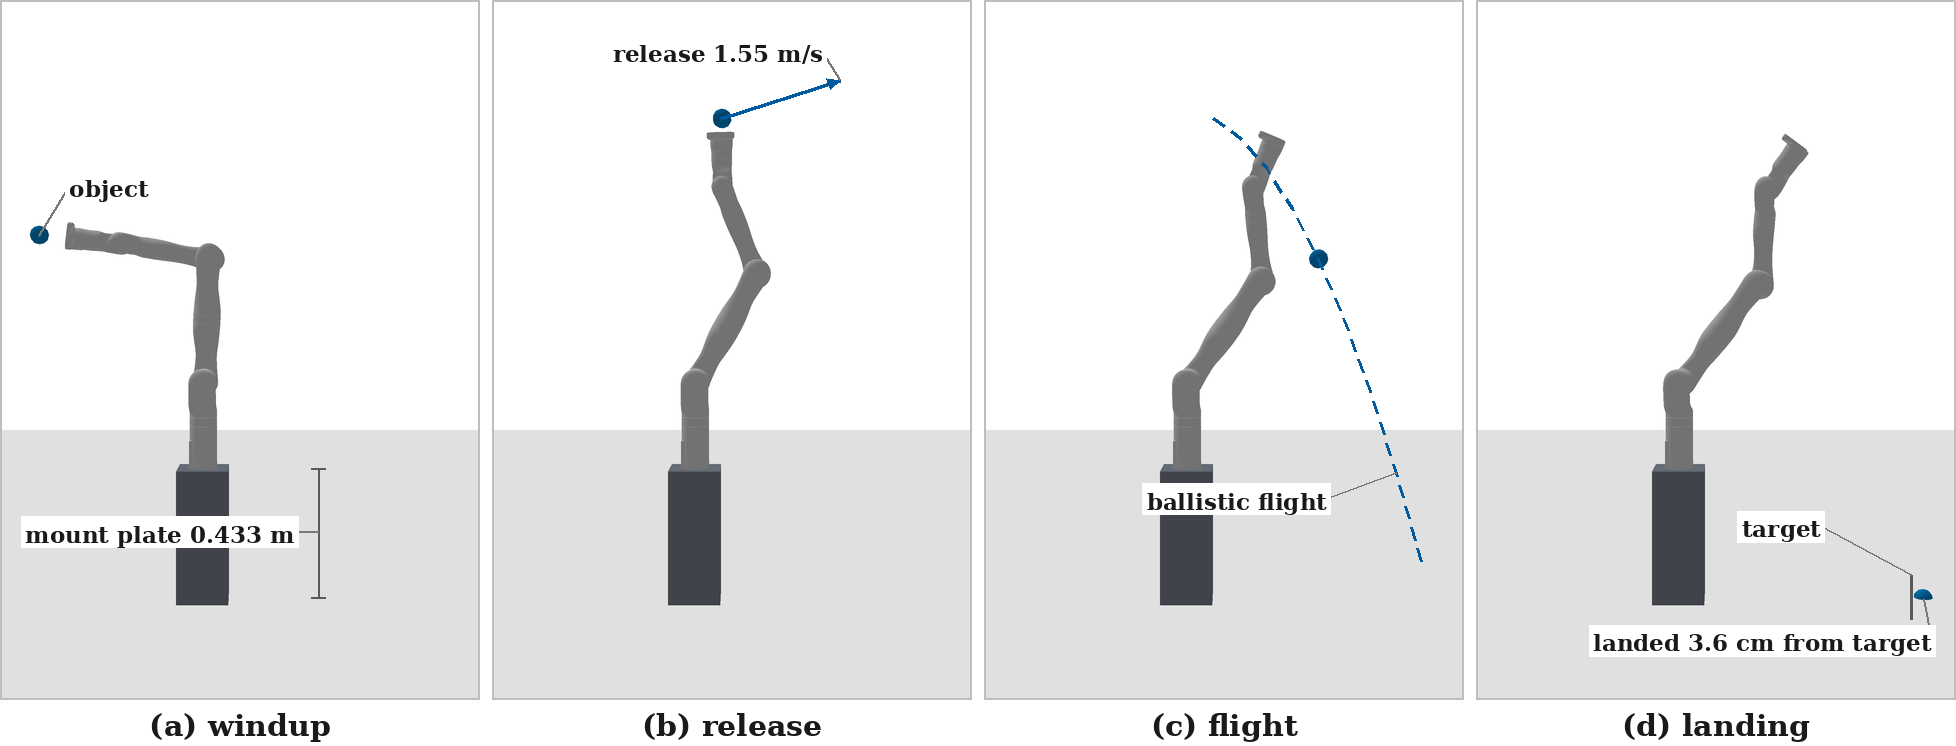
\includegraphics[width=\textwidth]{figs/fig_throw_snapshots.png}
\caption{Simulated Kinova Gen3 throw: (a) windup, (b) release, (c) flight
during post-release recovery, and (d) landing. Frames are from a single
rigid-body rollout of the learned policy under computed-torque control; the
dashed curve in (c) is the object's recorded trajectory.}
\label{fig:throw-phases}
\end{figure*}

\subsection{Dynamics-Aware Throw Execution}
\label{sec:method-torque}

The selected release state is evaluated using the coupled manipulator and
object dynamics. The manipulator is controlled using computed torque,
\begin{equation}
\tau =
M(q)\ddot q_{\mathrm{cmd}}
+
C(q,\dot q)
+
G(q)
+
J(q)^\top f_{\mathrm{ball}},
\label{eq:computed-torque}
\end{equation}
where $M$, $C$, and $G$ denote the mass, Coriolis/centrifugal, and gravity
terms, respectively. The payload compensation term is
\begin{equation}
f_{\mathrm{ball}}=m_{\mathrm{ball}}[0,0,g]^\top .
\end{equation}

The object is modeled as a separate rigid body attached through a removable
grip constraint. The attachment point is offset from the wrist flange by the
tool-center-point distance $r_{\mathrm{offset}}=0.12$~m. This offset is
included consistently in the release-state optimization and rigid-body
simulation. In particular, the release velocity contains the rotational
contribution
\begin{equation}
\mathbf{v}_{\mathrm{offset}}
=
\boldsymbol{\omega}\times r_{\mathrm{offset}},
\end{equation}
which would be omitted if the object were attached directly to the wrist
flange. The same attachment point is therefore used for release-state
calculation and simulation.

The release velocity is measured from the physics engine after the grip
constraint is removed rather than imposed directly. This ensures that the
reported release state corresponds to the velocity generated by the simulated
arm--object system.

\subsection{Target-Height Generalization}
\label{sec:method-height}

The target-conditioned formulation is extended to targets at different
heights by parameterizing both the trajectory termination plane and particle
propagation with the target height $h$. The policy input consequently becomes
$(P_x,P_y,h)$.

We consider three settings: training at a single fixed height, re-optimizing
the policy for discrete target heights while reusing the learned GP, and
training a single policy over a continuous range of target heights. The latter
tests whether the learned policy can interpolate to target heights not observed
during training without requiring a separate policy-optimization run for each
height.

%%%%%%%%%%%%%%%%%%%%%%_Results_%%%%%%%%%%%%%%%%%%%%%%
\section{Results and Discussion} \label{sec:results}
\subsection{Simulation Environment and Evaluation} \label{sec:setup-simulation}
All simulation experiments are conducted in PyBullet~\cite{coumans2021pybullet} using rigid-body dynamics and manufacturer-specified joint torque and velocity limits. We evaluate KUKA iiwa7, Franka Panda, xArm6, and Kinova Gen3 under the same model-based learning procedure, three seeds each, with only the arm model and its velocity limits varied; these four runs use each arm's prescribed release configuration, so they isolate the learning pipeline's arm-independence. The release-state search itself is run on the Kinova Gen3 and, in Sec.~\ref{sec:results-ablation}, the Franka Panda and UR7e. The Gen3 results are torque-controlled with the release velocity measured from the physics engine; the KUKA and Panda runs are position-controlled, and the xArm6 assigns the release velocity directly, so only the Gen3 numbers are physically realized throws. Gen3 targets are sampled in flight space relative to the actual release point. Final performance is evaluated on previously unseen targets and random seeds using complete rigid-body rollouts. Landing error is the Euclidean distance between the simulated landing position and the target. A throw counts as successful when this error falls below a stated threshold; we report two, a $10$~cm threshold matching the bin radius used in~\cite{turcato2025mcpilot} and a tighter $5$~cm threshold. Seed counts are stated with each result. Where conditions are compared against one another, they are evaluated on a single shared set of previously unseen targets, so that only the condition varies; comparisons across different manipulators are necessarily an exception, since each arm has its own reachable target band. 
\subsection{Hardware Environment} \label{sec:setup-hardware}
Hardware validation uses a 7-DOF Kinova Gen3 mounted approximately $0.433$~m above the floor. The planned trajectory is executed as a joint-velocity stream issued through the manufacturer's high-level real-time control interface, whose command rate is approximately 40~Hz. An Intel RealSense D435i provides visual sensing; the camera-to-base transform is recovered by observing a planar fiducial target of known dimensions and composing the resulting camera-to-target pose with the forward kinematics of the arm. Landing position is measured by triangulating the object in flight from the rectified infrared stereo pair and solving a ballistic fit for the descending crossing of the floor plane, rather than from block-matching depth, which is too noisy at this range for a small textureless sphere. The experiments are staged, each stage validated before the next is enabled. They cover state feedback, gripper actuation, velocity streaming, and object-loaded throws; the object's departure instant and its landing point remain unmeasured, so physical throwing accuracy is not evaluated.
\subsection{Training and Implementation Details} \label{sec:setup-implementation} 
The RBF policy length scale is initialized as \begin{equation} \ell_0=0.15(l_M-l_m), \end{equation} where $[l_m,l_M]$ is the target-distance range. The sparse GP uses $M=400$ inducing points and mini-batches of $N_b=250$. Simulation runs at 50~Hz and the Gen3 velocity interface at approximately 40~Hz. All remaining policy and dynamics parameters follow Sec.~\ref{sec:approach}.

%%%%%%%%%%%%%%%%%%%%%%%%%
%%%%%%%%%%%%%%%%%%%%%%%%%%%%

\subsection{Optimization Reliability}
\label{sec:results-baseline}

We first evaluate the reliability of model-based policy optimization across
random seeds. A single baseline run at a fixed seed achieves 5/5 successful
throws in five trials, at 1.81~cm mean landing error, which taken alone would
suggest the configuration is reliable. Repeating that same configuration over
five seeds instead yields hit rates of 60\%, 20\%, 80\%, 10\%, and 10\%,
indicating substantial sensitivity to initialization and exploration.

Two interacting factors account for this sensitivity. Unstratified exploration
can leave the GP poorly informed over parts of the release-speed range, while
an RBF lengthscale that is not scaled to the target domain can saturate the
policy response. Fig.~\ref{fig:reliability} separates the two: stratified
exploration alone recovers three of the five seeds, and only when it is
combined with target-range-scaled lengthscale initialization do all five
converge. Neither modification is therefore sufficient on its own.

With both modifications applied, the five seeds are evaluated on 50 previously
unseen targets each, yielding 250 throws. Every throw falls within both the
$<10$~cm and the $<5$~cm threshold, giving a 100\% hit rate at both, with a
mean landing error of 1.86~cm and a 95th-percentile error of 3.17~cm.
Fig.~\ref{fig:eval-dist} shows that this is consistent across seeds rather than
an average over dissimilar runs: per-seed mean error spans only
1.77--1.96~cm, and the worst single throw of all 250 is 3.81~cm, still inside
the tighter threshold.

\begin{figure}[t]
\centering
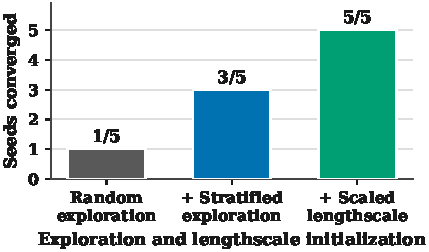
\includegraphics[width=\linewidth]{figs/fig_seed_reliability.pdf}
\caption{Seeds converged, out of five, under random exploration and under each
reliability modification in turn.}
\label{fig:reliability}
\end{figure}

\begin{figure}[t]
\centering
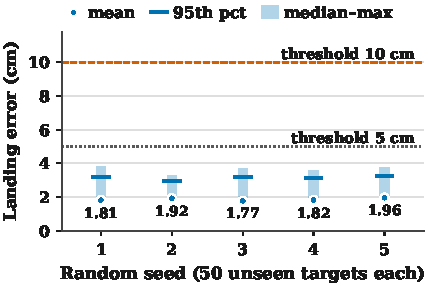
\includegraphics[width=\linewidth]{figs/fig_eval_spread.pdf}
\caption{Final-policy landing error per random seed, on 50 previously unseen
targets each.}
\label{fig:eval-dist}
\end{figure}


\subsection{Cross-Manipulator Evaluation}
\label{sec:results-multiarm}

The model-based learning pipeline is evaluated on KUKA iiwa7, Franka Panda,
xArm6, and Kinova Gen3 without arm-specific policy tuning beyond the
corresponding velocity limits. Mean landing error
ranges from 1.4 to 2.7~cm across the four manipulators, a spread comparable to
the seed-to-seed variation observed on a single arm in
Sec.~\ref{sec:results-baseline}. The learning pipeline is therefore not tied to the Gen3 geometry. Transfer of
the release-state search itself is a separate question, addressed on the Franka
Panda and the 6-DOF UR7e in Sec.~\ref{sec:results-ablation}.


\subsection{Aerodynamic-Drag Robustness}
\label{sec:results-drag}

We vary payload drag from less than 1\% to approximately 19\% of gravity and
compare the learned model with the analytical no-drag baseline. Three seeds per condition. Below $1\%$ drag the closed-form baseline is not
merely competitive but more accurate than the learned model (1.65 vs 1.86~cm on
the KUKA, 1.43 vs 1.94~cm on the Panda), since there is no unmodeled effect to
learn and learning still pays a variance cost. At $19\%$ drag the ordering
reverses by $4.3$--$4.6\times$ (5.34 vs 1.26~cm and 3.79 vs 0.82~cm).

We further vary payload mass from 30 to 150~g and diameter from 2 to 4.5~cm
without retraining. All twelve mass--diameter combinations remain within
1.38--1.46~cm mean landing error. The analytical model therefore remains
competitive when aerodynamic effects are small, while the learned dynamics
provide increasing benefit as the unmodeled drag becomes significant.

As an additional ablation, subtracting gravity as a GP mean function does not
improve accuracy: the mean error increases from 0.62 to 0.85~cm for the Panda
and from 1.69 to 1.77~cm for the KUKA. This suggests that imposing gravity as
the dominant structured component is not beneficial for the residual dynamics
in the tested regime.


\subsection{Target-Height Generalization}
\label{sec:results-height}

A single KUKA iiwa policy trained over a continuous target-height range is
evaluated on 100 fresh targets at heights not observed during training. It
records 100\% successful throws, a mean landing error of 2.13~cm, and a
worst-case error of 4.92~cm. Restricted to the three heights used in the
adaptation study below, the same policy gives 2.22, 2.03, and 2.12~cm mean
error at $h=0.10$, $0.20$, and $0.30$~m (targets within $\pm2.5$~cm of each
height; $n=4$, $18$, and $13$), showing no systematic trend with height.
Fig.~\ref{fig:height-gen} plots this error against
target height: the local mean stays between 1.7 and 3.0~cm across the entire
$0$--$45$~cm range, and in particular does not grow towards the boundaries of
the trained interval, so the single conditioned policy interpolates over height
rather than specializing to the centre of the range.

The preceding result uses a single policy conditioned on height and trained
over the whole interval. We next ask what happens when no such policy is
available, and evaluate zero-new-trial adaptation on the Gen3 overhead
configuration by reusing the trained GP and re-optimizing only the policy for
the same three target heights $h=0.10$, $0.20$, and $0.30$~m. The two studies
use different arms, so they bound different platforms rather than competing
with each other directly. Because each re-optimized policy selects its
own reachable target band, and those bands differ by more than an order of
magnitude in width, all four conditions are evaluated on a single fixed set of
30 previously unseen targets drawn from the intersection of the four bands, so
that target height is the only quantity that varies. On that shared set
(Fig.~\ref{fig:height-adapt}), mean landing error grows monotonically from
1.52~cm at ground level to 1.82, 2.24, and 2.40~cm at $h=0.10$, $0.20$, and
$0.30$~m, with every throw inside the 10~cm threshold and a worst case of
5.18~cm. A complete nine-dimensional retraining baseline is not included in
this comparison: the only such checkpoint on disk predates the gripper
tool-center-point correction of Sec.~\ref{sec:method-torque} and was trained
from a release point 0.39~m lower, so placing it alongside these numbers would
conflate that correction with the retraining-versus-adaptation question this
experiment is designed to isolate. Accuracy therefore degrades gradually and
predictably with height,
while adaptation costs no additional robot trials, so target-height changes can
be accommodated without relearning the GP dynamics.

\begin{figure}[t]
\centering
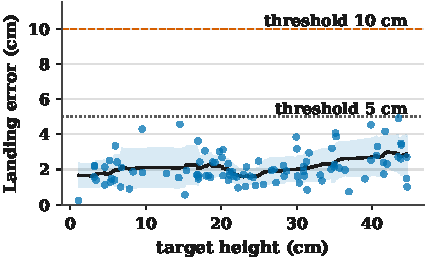
\includegraphics[width=\linewidth]{figs/fig_height_gen.pdf}
\caption{Landing error against target height for the KUKA iiwa, on 100 targets
at heights not seen during training. The line is a rolling mean, the band its
standard deviation.}
\label{fig:height-gen}
\end{figure}

\begin{figure}[t]
\centering
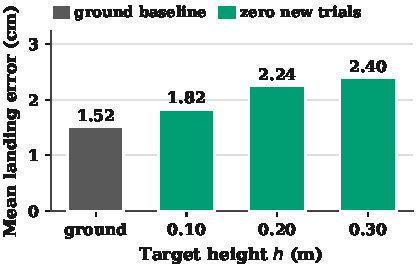
\includegraphics[width=\linewidth]{figs/fig_height_adaptation.pdf}
\caption{Zero-new-trial target-height adaptation on the Kinova Gen3, all
conditions evaluated on the same fixed set of 30 previously unseen targets.}
\label{fig:height-adapt}
\end{figure}


\subsection{Low-Torque Throwing}
\label{sec:results-overhead}

We next evaluate the release-state search on the low-torque Kinova Gen3. Under
a fixed low-release posture, increasing elevation reduces the achievable range,
causing distance optimization to favor a near-horizontal motion. In contrast,
searching over the release state under the complete feasibility cascade
identifies an overhead throwing configuration.

The selected configuration reaches a release height of approximately 1.1~m.
When windup, release, and post-release recovery constraints are enforced, the
maximum simulated safe-throw distance is 1.03~m, against the 0.75~m at which
this arm can place an object on the same floor -- it is mounted 0.433~m up, so
reaching down to floor level costs horizontal extent. Throwing therefore extends this arm's
floor-level placement radius by $1.4\times$. Over 30 previously unseen targets
the mean landing error is 1.52~cm, the worst case 3.70~cm, and every throw falls
within both thresholds. Release speed varies only from 1.35 to 1.47~m/s across
the target-distance range, well inside the arm's 2.07~m/s kinematic ceiling: the
trained target band, not the actuators, bounds the deployed policy.

% TODO(range-ceiling figure): held out pending reconciliation of the safe-throw
% and kinematic-reach numbers. The prose above (0.82 / 0.87 m) comes from the
% full posture-and-direction grid analysis reported in Table I; the regenerated
% figure below comes from paper_range_speed_sweep.py, which is a single-azimuth
% commanded-speed sweep and reports 0.70 / 0.94 m; a third, hand-made PNG that
% previously sat here reported 0.83 / 0.86 m. Uncomment once one of the three is
% adopted as canonical and the others are brought into line -- and add the
% sentence describing the dashed segment back into the paragraph above.
% \begin{figure}[t]
% \centering
% 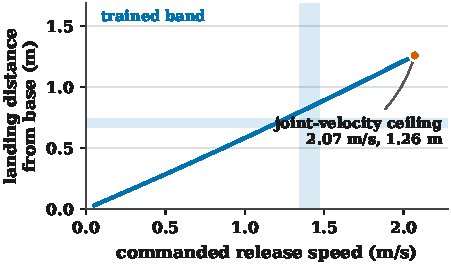
\includegraphics[width=\linewidth]{figs/fig_range_ceiling.pdf}
% \caption{Landing distance against commanded release speed for the Kinova Gen3.
% The dashed segment is reachable but fails the post-release recovery check.}
% \label{fig:range-ceiling}
% \end{figure}


\subsection{Whole-Trajectory Feasibility}
\label{sec:results-ablation}

We quantify the importance of whole-trajectory feasibility by applying the same
release-pose and direction enumeration to the Gen3 and Franka Panda. Candidates
that satisfy the release-instant criterion are subsequently evaluated using the
complete feasibility cascade. The resulting counts are summarized in
Table~\ref{tab:ablation}.

\begin{table}[t]
\centering
\small
\caption{Release-instant-only versus whole-trajectory feasibility across three
manipulators on the same posture and direction grid. Bodyless frames in each
manipulator description are given zero mass; loading the Gen3 description
unmodified instead assigns them the simulator's 1~kg default, adding 3.00~kg at
the wrist and reducing its survivors to 74{,}230 (16.6\%).}
\label{tab:ablation}
\begin{tabular}{@{}lccc@{}}
\toprule
 & Gen3 & Panda & UR7e \\
\midrule
Release-instant-feasible & 475{,}123 & 152{,}844 & 541{,}590 \\
Also full-traj.-feasible & 391{,}238 & 152{,}844 & 541{,}569 \\
                         & (82.3\%) & (100\%) & (100.0\%) \\
Rej.\ windup-path & 0 & 0 & 0 \\
Rej.\ throw-ramp & 0 & 0 & 0 \\
Rej.\ follow-through & 83{,}885 (17.7\%) & 0 & 21 \\
Best range, instant-only & 1.03~m & 1.65~m & 2.55~m \\
Best range, full check & 1.03~m & 1.65~m & 2.55~m \\
\bottomrule
\end{tabular}
\end{table}

For the Gen3, 391{,}238 of 475{,}123 release-instant-feasible candidates remain
feasible after the complete cascade. Every rejection is attributed to the
post-release follow-through: at this arm's real torque limits, no candidate that
reaches the release state fails on the windup path or the throw ramp. The
rejected 17.7\% is therefore a recovery constraint rather than a torque
shortfall, and the sweep below shows that no additional actuator capacity
removes it. The best achievable range is unchanged at 1.03~m, because the
range-optimal candidate is itself whole-trajectory feasible: the cascade
determines \emph{which} release state is selected and whether the selected
motion is executable, not how far the arm can throw.

For the Panda and the UR7e essentially every release-instant-feasible candidate
also satisfies the cascade (100\% and 99.996\%), and neither maximum range
moves. The cascade is thus cheap insurance on an arm with actuator headroom and
decisive on one without, which is the argument for applying it unconditionally. Because the Gen3
and Panda differ in both kinematics and torque limits, their direct comparison
does not isolate the effect of actuator torque. We therefore repeat the
analysis using Gen3-identical kinematics and control gains while scaling only
the torque limits by a factor $k$ (Fig.~\ref{fig:torque-sweep},
Table~\ref{tab:torque-sweep}).

\begin{figure}[t]
\centering
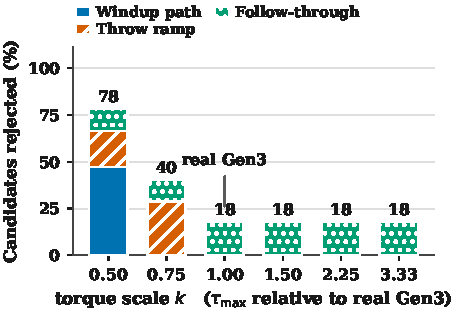
\includegraphics[width=\linewidth]{figs/fig_torque_sweep.pdf}
\caption{Share of release-instant-feasible candidates rejected by each stage of
the cascade, against actuator torque capacity, for Gen3-identical kinematics.}
\label{fig:torque-sweep}
\end{figure}

\begin{table}[t]
\centering
\small
\caption{Torque-capacity sweep using Gen3-identical kinematics. Rejection rates
are computed relative to the torque-dependent release-instant-feasible pool.}
\label{tab:torque-sweep}
\begin{tabular}{@{}lrrrr@{}}
\toprule
$k$ & wrist $\tau_{\max}$ & instant- & full-traj- & rej. \\
    & (Nm)                & feasible & feasible   & (\%) \\
\midrule
0.50 & 4.5   & 444{,}713 & 96{,}584  & 78.3 \\
0.75 & 6.75  & 475{,}123 & 284{,}156 & 40.2 \\
1.00\rlap{$^{\dagger}$} & 9.0 & 475{,}123 & 391{,}238 & 17.7 \\
1.50 & 13.5  & 475{,}123 & 391{,}238 & 17.7 \\
2.25 & 20.25 & 475{,}123 & 391{,}238 & 17.7 \\
3.33\rlap{$^{\ddagger}$} & 29.97 & 475{,}123 & 391{,}238 & 17.7 \\
\bottomrule
\end{tabular}

\vspace{2pt}
{\footnotesize $^{\dagger}$reproduces the real Gen3 torque limits.
$^{\ddagger}$approximates the Panda torque ratio only and does not reproduce
its kinematics.}
\end{table}

Fig.~\ref{fig:torque-sweep} decomposes this rejection by cascade stage, and the
three stages bind in sequence rather than together. At $k=0.50$ the windup path
dominates (47.3\% of the pool), with throw ramp and follow-through at 19.0\% and
12.0\%: the arm struggles to reach a throwing posture at all. By $k=0.75$ the
windup path clears and the throw ramp binds at 28.7\%. From $k=1.00$ both clear
and rejection saturates at 17.7\%, entirely follow-through. Saturation therefore
begins exactly at the real Gen3's own torque limits: this arm is not
torque-starved for the throw itself, its binding constraint is already the
recovery motion, which is kinematic in origin and unaffected by additional
torque.


\subsection{Computational Efficiency}
\label{sec:results-cost}

A complete Gen3 overhead-throw training run with 10 trials, including five
exploration trials and $N_{\mathrm{opt}}=1500$ policy-optimization steps per
trial, requires 17~min~44~s on a single CPU core with 1.11~GB peak memory. The
one-time release-state search enumerates $3.2\times10^{4}$ release postures
against six candidate directions each and requires 28~min~27~s on the same
machine, at a single azimuth that is then propagated by base rotation. These
costs are incurred once per arm and workspace geometry, after which the
release-state table is reused across training seeds and evaluation targets.


\subsection{Hardware Validation}
\label{sec:results-hw}

The physical Kinova Gen3 is used to validate the unloaded execution pipeline.
Table~\ref{tab:hw-status} records how far that validation has progressed: each
row is one capability the execution stack requires, and the pipeline is
enabled one row at a time, so the two rows still marked pending are precisely
what separates the present hardware study from a measured physical throw.
State read-back, gripper actuation, full-speed joint-velocity streaming, and
object-loaded throws have all been executed on the physical arm; what is not yet
measured is when the object leaves the hand and where it lands.

Joint angles are handled using the $[0^\circ,360^\circ)$ convention reported by
the arm. Across $n=9$ full-speed throws the arm lags the commanded profile by about one
control interval: at the planned release instant the measured tool-centre speed
is $0.948\pm0.005$ of commanded, the direction $3.82\pm0.47^\circ$ steeper, and
joint drift $0.037\pm0.004$~rad, which propagate ballistically to
$10.2\pm0.9$~cm short of plan. Gripper-open onset is $67.9\pm6.7$~ms ($n=15$,
empty) and $66.9\pm15.2$~ms ($n=3$, on a ball) with the stream idle, and the
executor leads the open command by that latency. In-throw recordings show the
lead is ineffective: while joint velocities stream the fingers do not move, and
across $n=4$ instrumented throws they first moved $49$--$74$~ms \emph{after} the
planned release instant. The two dominant terms then oppose -- during the stream
pause the arm coasts at its held release velocity, so a late departure flattens
the release and lengthens the throw while the command lag shortens it.
Fig.~\ref{fig:error-budget} plots the net error against departure instant:
$-10.2$~cm at onset, crossing zero at $65$~ms. Neither can be corrected alone
without risking a larger error of the opposite sign, and the 25~ms command
interval sets a $3.6$~cm floor beneath both.

\begin{table}[t]
\centering
\small
\caption{Which stages of the execution pipeline have run on the physical Kinova Gen3. What separates this study from a physical accuracy result is measurement, not execution.}
\label{tab:hw-status}
\begin{tabular}{@{}p{4.9cm}c@{}}
\toprule
Execution stage & Executed on the arm \\
\midrule
Read joint and gripper state & yes \\
Command the gripper & yes \\
Stream joint velocities at full speed & yes \\
Keep open-loop drift within budget & yes \\
Throw with the object in the gripper & yes \\
Compensate gripper latency at release & attempted, ineffective \\
Measure the object's departure instant & not yet \\
Measure the physical landing point & not yet \\
\bottomrule
\end{tabular}
\end{table}

\begin{figure}[t]
\centering
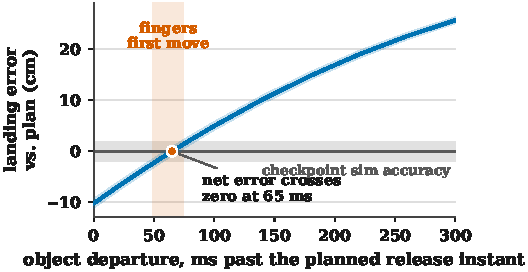
\includegraphics[width=\linewidth]{figs/fig_error_budget.pdf}
\caption{Net landing error against the instant the object leaves the hand,
from $n=9$ recorded full-speed throws (band: $\pm1$ s.d.). The command lag makes
the throw short and a late release makes it long, so the two cancel near
$65$~ms; the shaded column is where the fingers were observed to first move.}
\label{fig:error-budget}
\end{figure}

These measurements establish the operation of the hardware execution stack at
the full planned release speed. This
exceeds the manufacturer's documented 0.500~m/s Cartesian speed ceiling, but
that ceiling applies to a Cartesian control mode distinct from the joint-space
velocity streaming used here, as confirmed both by the arm's reported mode
limits and by a full-speed empty-gripper rehearsal completing without fault.
What remains is measurement, not execution: the object's departure instant and
its landing point are both unresolved, so no physical landing accuracy is
claimed.


\subsection{Discussion}
\label{sec:discussion}

The results support three main conclusions. First, on an arm whose actuators cannot realize a prescribed release
configuration, searching the release state is what makes the throw exist at all:
the Gen3's prescribed posture drives distance optimization toward a
near-horizontal push, and the search recovers a genuine overhead throw. Second,
whole-trajectory feasibility matters most near actuator limits, but not for the
reason a release-instant analysis suggests: at the Gen3's real torque limits
neither the windup path nor the throw ramp rejects anything, and the only
binding stage is the post-release recovery, which the torque sweep shows to be
kinematic in origin and unaffected by added actuator capacity. Third, model-based
learning becomes increasingly beneficial as the analytical no-drag model
departs from the observed dynamics, while target-height conditioning enables
adaptation without relearning the GP dynamics.

The results also clarify the role of the proposed framework. It does not remove
the physical limits of the manipulator; rather, it identifies and exploits the
subset of release states for which the complete throwing motion remains
executable. The achievable throwing range is therefore jointly determined by
kinematic reach, actuator torque, joint velocity, and post-release recovery
constraints.

Five limitations bound these conclusions. The accuracy results are established
in rigid-body simulation; the physical arm executes the full stack including
object-loaded throws, but the object's departure instant and its landing point
are both unmeasured, so no physical accuracy is claimed. The feasibility counts
depend on whether bodyless frames in the manipulator description are given zero
mass, which changes them fivefold on the Gen3 and not at all on the Panda. The release-state search is a discrete enumeration and therefore
incurs a one-time computational cost that depends on grid resolution. Object
and multi-manipulator generalization are currently evaluated in simulation, and
the shared computed-torque gains have not been independently validated for each
arm. In addition, the Gen3 implementation uses fixed lead-time compensation
for measured gripper delay rather than learning a release-delay distribution.
Finally, the current hardware study does not yet establish how the measured
timing and drift effects combine during a physical loaded throw.


\section{Conclusion}
\label{sec:conclusion}

We presented a constraint-aware model-based framework for robotic PTP in which the release state is selected according to the manipulator's kinematic and dynamic capabilities rather than fixed a priori. The framework combines arm-specific release-state search and whole-trajectory feasibility checking with Gaussian-process dynamics learning and particle-based policy optimization, enabling target-dependent throwing within the feasible operating envelope.

Across four simulated manipulators the learning pipeline yields 1.4--2.7~cm mean landing error without arm-specific policy tuning, and the release-state search transfers to a 6-DOF UR7e without algorithmic change. On the low-torque Kinova Gen3 it identifies a 1.03~m safe-throw boundary against the 0.75~m at which the same arm can place an object on that floor, at 1.52~cm mean landing error on previously unseen targets. The additional drag and target-height experiments show that learned dynamics become increasingly beneficial when analytical dynamics are incomplete, while target-conditioned policies can adapt to unseen target heights without relearning the GP dynamics.

Physical Gen3 experiments exercise the execution stack end to end with an object in the gripper and quantify the release-timing terms that govern transfer. Measuring the object's departure instant and its landing point remains to be completed, together with broader real-world validation across manipulators and object conditions. Future work will therefore focus on physical throwing evaluation, improving the efficiency of the release-state search, and extending the framework to broader robot and object configurations. Thus, the present work establishes the simulation-side effectiveness and hardware execution readiness of the proposed constraint-aware formulation, with full real-world throwing evaluation left as the next step.



%%%%%%%%%%%%%%%%%%%%%%%%%%%%%%%%%%%%%%%%%%
\bibliographystyle{ieeetr}
\bibliography{reference}

\end{document}


%%%%%%%%%%%%%%%%Earlier_draft%%%%%%%%%%%%%%%%%%%%%
%%%%%%%%%%%%%%%%%%%%%%%%%%%%%%%%%%%%%%
%%%%%%%%%%%%%%%%%%%%%%%%%%%%%%%%%%%%%%%%%
%%%%%%%%%%%%%%%%%%%%%%%%%%%%%%%%%%%%%%%%%%%%%%%%%%%%%%%%%%%%%%%
% \documentclass[letterpaper, 10 pt, conference]{ieeeconf}
% \IEEEoverridecommandlockouts
% \usepackage{graphicx}
% \usepackage{amsmath}
% \usepackage{amssymb}
% \usepackage{amsfonts}
% \usepackage{booktabs}
% \usepackage{xcolor}
% \usepackage{url}
% % A figure* placed right after \maketitle silently defers to page 2 in this
% % class (\maketitle zeroes the top-of-page float counters as part of its own
% % \twocolumn[...] title block) -- neither [t!] nor dblfloatfix nor bumping
% % \dbltopfraction override that. The class's own documented escape hatch is
% % \IEEEaftertitletext{}: content injected there renders as part of the
% % guaranteed single-column title block itself, not as a float, so it cannot
% % be deferred. capt-of gives it a normal numbered "Fig. 1" caption outside
% % a float environment.
% \usepackage{capt-of}


% %%%%%%%%%%%%%%%%%%%%%%%%%%%%%%%%%%%%%%%%%%%%%%%%%%%%
% \title{\LARGE \bf
% Enabling Pick-and-Throw on Low-Torque Manipulators through Constraint-Aware Data-Efficient Model-Based Learning
% }
% \author{Anonymous submission}

% %\author{ Dharmendra Sharma, Rohit Jangra, Deepak Raina, Narendra Kumar Dhar}
% %\IEEEauthorblockA{Indian Institute of Technology Mandi, India}

% \begin{document}

% \IEEEaftertitletext{%
% \begin{center}%
% 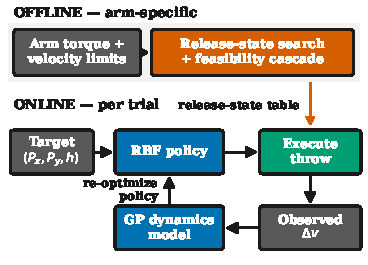
\includegraphics[width=0.78\textwidth]{figs/fig_pipeline.pdf}\\[2pt]
% {\small\captionof{figure}{System overview. \emph{Offline, once per arm}
% (top): the release state is searched under the arm's real torque and
% velocity limits and validated by the whole-trajectory feasibility cascade,
% producing a release-state table. \emph{Online, per trial} (bottom): a
% target-conditioned RBF policy outputs a release speed, executed through that
% same table; the resulting flight is used to update a Gaussian-process
% dynamics model, against which the policy is re-optimized offline before the
% next trial.}\label{fig:pipeline}}%
% \end{center}%
% \vspace{-4pt}%
% }

% \maketitle

% %%%%%%%%%%%%%%%%%%%%%%%%%%%%%%%%%%%%%%%%%%%%%%%%%%%%%%%%%%%%%%%%%%%%%%%%%%%%%%%%
% \begin{abstract}
% Robotic pick-and-throw extends a manipulator's reach for tasks such as sorting and material handling, but executing an accurate release is difficult on manipulators with limited torque and velocity headroom. Model-based reinforcement learning (MBRL) enables data-efficient pick-and-throw from a small number of physical trials, but existing approaches assume a predefined release configuration, which can be infeasible on such manipulators. This paper presents a constraint-aware extension of model-based pick-and-throw in which the release state is explicitly searched under kinematic, torque, and joint-velocity constraints. Instead of validating only the release instant, we evaluate the complete windup, throw, and post-release follow-through trajectories, thereby accounting for dynamic constraints that can otherwise produce infeasible releases. The resulting release-state search is integrated with a Gaussian-process dynamics model and particle-based policy optimization; the same release-planning logic used during training also drives hardware execution. Across four simulated manipulators, the proposed approach achieves 1.4--2.7~cm mean landing error without per-arm policy tuning beyond the corresponding torque and velocity limits. On the Kinova Gen3, the analysis identifies a measurable 0.82~m safe-throw range under the full-trajectory feasibility constraints. We further show that a single policy can generalize across a continuous range of target heights and characterize a drag regime in which model-based learning provides a 3--7-fold accuracy improvement over a no-drag analytical baseline. Hardware experiments on the Gen3 validate the unloaded stages of the execution pipeline, including state feedback, gripper actuation, and full-speed joint-velocity streaming.
% \end{abstract}

% \begin{keywords}
% Pick-and-throw, model-based RL, Gaussian process
% regression, manipulator dynamics, dynamic nonprehensile manipulation
% \end{keywords}

% \section{Introduction}

% Pick-and-throw (PnT) is a complementary alternative to pick-and-place: releasing an object with a controlled velocity lets a robot reach beyond its end-effector workspace, faster than a full place motion allows. Accurate throwing requires a sufficiently fast release within the arm's kinematic and dynamic limits -- small errors in release position, velocity, or timing produce large landing errors at speed.

% Recent work has shown that model-based reinforcement learning (MBRL) can make robotic throwing substantially more data efficient. MC-PILOT~\cite{turcato2025mcpilot}, for example, combines sparse Gaussian-process (GP) dynamics learning with particle-based policy optimization and achieves accurate throwing from only a small number of physical trials. A key design choice in that framework is to use a predefined release configuration: the learned policy determines the throwing direction and release speed, while the joint trajectory leading to the release state is fixed analytically. This decomposition reduces the dimensionality of policy optimization and is effective on the Franka Emika Panda considered in the original study.

% A fixed release configuration, however, implicitly assumes that the selected manipulator has sufficient actuator capability to realize the desired release motion. This assumption becomes restrictive for lower-torque manipulators. In our experiments with the 7-DOF Kinova Gen3, whose wrist actuators provide substantially less torque than those of the (also 7-DOF) Franka Panda, directly adopting the fixed-release strategy does not produce a useful throw. Under the predefined release posture, increasing the release elevation reduces the achievable range, causing distance-based optimization to favor a near-horizontal motion rather than a genuine throw. This observation motivates a different formulation: rather than treating the release configuration as a fixed design choice, the release state itself should be selected according to the capabilities of the robot.

% We therefore formulate release-state selection as a constraint-aware search over robot posture and release direction, with the maximum achievable release speed obtained under joint-velocity constraints and each candidate evaluated by a feasibility cascade over the complete windup-to-follow-through motion -- not just the release instant, since a release state can satisfy torque limits there while violating them elsewhere in the motion. This search is performed once per robot and workspace, then combined with the MBRL policy, which learns the target-dependent release speed from the observed throwing dynamics.

% The resulting framework is evaluated in rigid-body simulation on four manipulators: KUKA iiwa7, Franka Panda, xArm6, and Kinova Gen3. Across these platforms, the constraint-aware release-state search achieves 1.4--2.7~cm mean landing error without per-arm policy tuning beyond the corresponding torque and velocity limits. On the Gen3, whole-trajectory feasibility reduces the maximum recoverable throwing range relative to a release-instant-only analysis, revealing a measurable 0.82~m safe-throw ceiling under the considered configuration and constraints. We further demonstrate continuous target-height generalization, with a single policy achieving 2.0~cm mean landing error on previously unseen target heights. Finally, experiments over different drag regimes show that the analytical no-drag model is competitive when drag is negligible, whereas model-based learning provides a 3--7-fold reduction in landing error when drag becomes significant.

% Our contributions are as follows:
% \begin{enumerate}

% \item Constraint-aware release-state search: We propose a robot-specific search over release posture and direction that replaces the fixed release configuration, subject to joint-velocity and dynamic constraints.

% \item Whole-trajectory feasibility analysis: We introduce a feasibility cascade that evaluates windup, throw, and post-release follow-through motions rather than checking only the release instant, and quantify its effect on the feasible throwing range.

% \item Generalization and model-analysis study: We demonstrate continuous target-height generalization and characterize the operating regime in which model-based learning provides an advantage over a no-drag analytical model.

% \item Multi-manipulator evaluation and hardware validation: We evaluate the same release-state search and learning pipeline across four simulated manipulators and validate the unloaded components of the execution pipeline on a real Kinova Gen3.
% \end{enumerate}

% \section{Related Work}

% \subsection{Analytical throwing}
% Analytical throwing methods derive release conditions from a ballistic or
% kinematic model of the object and manipulator. The foundational treatment of
% throwing as a form of dynamic nonprehensile manipulation, alongside catching
% and batting, is given by Lynch and Mason~\cite{lynch1999dynamic}, who
% analyze the controllability and planning of motions that exploit gravity and
% momentum rather than a force-closure grasp. Such analytical approaches can
% provide fast and interpretable solutions when the relevant dynamics are
% accurately known, but their performance depends on the validity of the
% underlying model and on the available actuator capabilities.

% \subsection{Model-free learning}
% TossingBot~\cite{zeng2020tossingbot} learns a throwing policy from outcome
% data using residual physics. Its formulation demonstrates that throwing can
% be learned directly from robot interaction, but requires substantially more
% physical trials than model-based approaches. TossingBot also fixes the
% release direction and learns the release speed, reducing the dimensionality
% of the action space. Munn et al.~\cite{munn2024wholebody} instead address
% actuator-limited throwing by recruiting additional degrees of freedom: a
% legged manipulator learns, via deep reinforcement learning, to coordinate
% whole-body momentum with the arm, extending achievable release speed beyond
% what the arm alone provides.

% \subsection{Model-based learning}
% MC-PILOT~\cite{turcato2025mcpilot} combines sparse Gaussian-process dynamics
% learning with particle-based policy optimization and achieves data-efficient
% throwing on a Franka Panda, building on the MC-PILCO model-based
% policy-search algorithm~\cite{amadio2022mcpilco} and an earlier
% model-based tossing formulation~\cite{turcato2023codit}. Its formulation
% learns the target-dependent release speed while using a predefined release
% configuration and a hand-designed swing trajectory. The approach also
% demonstrates adaptation to different target heights by re-optimizing the
% policy using the already learned dynamics model.

% Our work addresses limitations that arise when this design is transferred to
% a manipulator with less actuator headroom. Specifically, we make the release
% state itself a search variable, impose torque and velocity constraints over
% the complete throwing motion, and evaluate the reliability and
% generalization of the resulting model-based policy across multiple
% manipulators, target heights, and drag conditions.

% \subsection{Constraint-aware motion generation}
% Manipulator trajectory optimization commonly incorporates joint-position,
% velocity, acceleration, and torque constraints. Such constraints are
% particularly important for high-speed motions, where satisfying limits at a
% single configuration does not guarantee feasibility along the trajectory.
% Two recent examples address this directly for throwing: Werner et
% al.~\cite{werner2024dynamic} learn a reinforcement-learning controller that
% exploits the passive joints of an underactuated, torque-limited
% material-handling machine to execute dynamic throws beyond its static
% reach, validated on a real 12-ton platform; Liu et
% al.~\cite{liu2022adaptive} reduce the throwing problem to a planar
% feasibility model that a mobile manipulator solves in real time, allowing
% the release motion to be replanned online under disturbance. Our formulation
% instead filters candidate release states offline through a staged
% feasibility cascade over the windup, release acceleration, and post-release
% recovery -- reused during policy learning, not a general-purpose trajectory
% optimizer.

% \section{Constraint-Aware Model-Based Pick-and-Throw}

% \subsection{Problem Formulation and Learning Framework}
% Following MC-PILOT~\cite{turcato2025mcpilot}, we formulate pick-and-throw as
% a model-based policy-search problem. A sparse Gaussian-process (GP) model
% approximates the object's velocity dynamics from collected transitions, and
% particle-based policy optimization searches for a target-conditioned release
% speed. The main modification is that the release configuration is no longer
% fixed a priori. Instead, we first determine a release state that is
% kinematically and dynamically feasible for the selected manipulator.

% The complete pipeline therefore consists of three stages. First, a
% robot-specific release-state search determines a feasible release posture,
% direction, and maximum achievable release speed. Second, the resulting
% release-state table is integrated with the GP-based policy optimization.
% Third, the learned policy is evaluated using a rigid-body simulation of the
% complete arm and object dynamics rather than using the training-time particle
% cost alone. The same release solver is used for simulation and hardware
% execution.

% Following~\cite{turcato2025mcpilot}, the object dynamics are represented by
% three independent sparse GPs, one for each Cartesian velocity component.
% Each GP is trained using transitions of the form
% $(\text{position},\text{velocity})\rightarrow\Delta\text{velocity}$
% collected from throwing trials. An RBF policy maps the target position, and
% in the height-generalized formulation the target height, to a release speed.

% The policy output is constrained to $[0,u_M]$ using
% \begin{equation}
% u =
% \frac{u_M}{2}\left(\tanh(x)+1\right),
% \end{equation}
% where $x$ is the unconstrained policy output. During policy optimization,
% particles are propagated through the learned GP dynamics and the policy is
% updated to minimize expected landing distance. Because optimization is
% performed against the learned model, policy improvement between physical
% trials does not require additional robot interaction.

% \subsection{Release-State Optimization}
% \label{sec:method-search}

% The original formulation fixes the release joint configuration
% $q_{\mathrm{rel}}$ and learns only the target-dependent release speed and
% aiming variables. We instead search over the release state
% $(q,\dot q)$. The search has two levels: an outer enumeration over candidate
% release postures and directions, and an inner optimization that determines
% the maximum release speed achievable at each candidate.

% \textbf{Inner release-speed optimization.}
% For the 7-DOF Gen3, the three pitch joints provide the dominant contribution
% to velocity perpendicular to the selected swing plane. The four
% roll/twist joints are therefore held at zero velocity during release-state
% optimization:
% \begin{equation}
% \begin{aligned}
% \max_{\dot q,s}\quad &s\\
% \text{s.t.}\quad &J(q)\dot q=s\hat d,\\
% &|\dot q_i|\leq\dot q_i^{\max},\qquad \forall i,\\
% &\dot q_i=0,\qquad i\in\{0,2,4,6\}.
% \end{aligned}
% \label{eq:release-lp}
% \end{equation}
% Here, $s$ is the release speed and $\hat d$ is the desired unit release
% direction. The problem is linear in $(\dot q,s)$ and is solved using
% \texttt{scipy.optimize.linprog} with the HiGHS solver.

% The static angles of the roll/twist joints remain free search variables.
% They are not assigned velocities because allowing them to contribute to
% release motion can produce a rotational motion that is poorly aligned with
% the desired throwing direction. A nonzero static offset also prevents the
% pitch axes from becoming geometrically degenerate.

% \textbf{Outer posture and direction search.}
% Candidate release postures are obtained by grid-searching the relevant joint
% angles and static offsets. For each posture, we first check minimum
% end-effector height and static gravity-induced torque feasibility. Candidate
% release directions are then sampled within the posture-dependent swing plane,
% using elevation angles from $5^\circ$ to $45^\circ$ at $5^\circ$ increments
% and both elevation signs.

% For every surviving posture-direction pair, the inner optimization in
% Eq.~\eqref{eq:release-lp} determines the maximum feasible release speed.
% Candidates are subsequently evaluated by the complete feasibility cascade
% described in Sec.~\ref{sec:method-feasibility}. Among candidates that pass
% all checks, the release state that maximizes the true landing distance is
% selected. Landing distance is computed by forward integration of the
% drag-augmented ballistic dynamics from the candidate's actual release
% position and velocity.

% \subsection{Azimuth Propagation}

% Once verified for a given arm and workspace, the release state is
% propagated over the required base-azimuth range by rotating the base joint:
% because gravity is invariant under rotation about the vertical axis, the
% Jacobian and feasibility properties rotate consistently with the base
% angle, so we construct an azimuth-to-pose table rather than independently
% optimizing every azimuth.

% For the Gen3, the verified release state is propagated over a
% $-33^\circ$ to $+33^\circ$ azimuth range at $3^\circ$ increments. A
% turret-aiming correction accounts for the offset between the tabulated
% release geometry and the target bearing. The same
% \texttt{OptimizedReleaseSolver} is used during training and execution; a
% regression test asserts that the simulation and hardware planners agree to
% within $10^{-12}$ on the resulting release state.

% \subsection{Whole-Trajectory Feasibility}
% \label{sec:method-feasibility}

% Release-instant feasibility alone does not guarantee that the complete
% throwing motion can be executed within the manipulator's limits. We
% therefore evaluate each candidate using four sequential checks. A candidate
% is rejected at the first stage that it fails.

% \begin{enumerate}
%     \item \textbf{Kinematic windup bound.}
%     The windup configuration
%     \begin{equation}
%     q_{\mathrm{windup}}
%     =
%     q_{\mathrm{rel}}
%     -
%     \dot q_{\mathrm{rel}}\frac{t_{\mathrm{throw}}}{2}
%     \end{equation}
%     must satisfy all joint-position limits.

%     \item \textbf{Windup-path torque.}
%     We sample the neutral-to-windup motion and evaluate gravity-induced
%     inverse dynamics at five intermediate configurations. Torque must remain
%     below $90\%$ of the corresponding manufacturer limit.

%     \item \textbf{Throw-ramp torque.}
%     The exact cubic windup-to-release velocity profile used by the runtime
%     controller is evaluated at 40 points. In addition to inverse dynamics,
%     the calculation includes the Jacobian-transpose feedforward term
%     associated with the gripped object's weight. The resulting torque must
%     remain below $75\%$ of the corresponding limit.

%     \item \textbf{Follow-through torque and velocity.}
%     The post-release recovery motion is evaluated over eight candidate
%     recovery durations from $0.6$ to $4.0$~s, with 30 samples per duration.
%     Both torque and joint velocity limits are checked. A candidate is
%     accepted if at least one recovery duration satisfies the specified
%     margins.
% \end{enumerate}

% This cascade explicitly accounts for failure modes that are invisible to a
% release-state-only check. In particular, a candidate can satisfy torque
% constraints at release while violating them during the windup or while
% recovering from a high-speed release.

% \subsection{Dynamics-Aware Throw Execution}
% \label{sec:method-torque}

% To evaluate the release state through the arm and object dynamics, the
% simulated manipulator is controlled using computed torque:
% \begin{equation}
% \tau =
% M(q)\ddot q_{\mathrm{cmd}}
% +
% C(q,\dot q)
% +
% G(q)
% +
% J(q)^\top f_{\mathrm{ball}},
% \label{eq:computed-torque}
% \end{equation}
% where $M$, $C$, and $G$ denote the manipulator mass, Coriolis/centrifugal,
% and gravity terms, respectively. The final term explicitly compensates for
% the weight of the gripped object:
% \begin{equation}
% f_{\mathrm{ball}}=m_{\mathrm{ball}}[0,0,g]^\top.
% \end{equation}
% The ball is modeled as a separate rigid body attached through a removable
% grip constraint. The explicit feedforward term therefore accounts for the
% payload even though it is not part of the manipulator's kinematic chain.

% The attachment point is offset from the wrist flange by the gripper's tool
% center point, $r_{\mathrm{offset}}=0.12$~m, applied consistently to the
% release-speed optimization (Eq.~\eqref{eq:release-lp}, Jacobian evaluated at
% the tool point) and to the simulation, where the ball is welded at the same
% point. Because the wrist is rotating at release, this offset contributes an
% additional velocity component $\omega\times r_{\mathrm{offset}}$ that a
% flange-attached model omits -- approximately $+0.39$~m/s ($+26\%$) and a
% $1.24^\circ$ direction change at the release state where this was measured.
% Placing the attachment point correctly reproduces this contribution
% directly from the rigid-body physics, without a manually derived
% correction term.

% Release velocity is measured from the physics engine after the
% grip constraint is removed rather than assigned directly. This ensures that
% the reported release velocity corresponds to the velocity actually produced
% by the simulated arm.

% Three further mismatches were fixed during validation: targets are sampled
% in flight space around the release point, not the base origin, which
% produced unreachable off-axis targets; the particle model uses the
% empirical mean release position from collected trials, not the nominal one;
% and the windup trajectory is rendered and checked to rule out a
% zero-amplitude windup.

% \subsection{Height-Generalized Policy}

% To evaluate generalization beyond a single landing plane, both the
% trajectory-termination plane and particle propagation are parameterized by
% the target height $h$. The policy input is therefore
% $(P_x,P_y,h)$. We compare three settings: a policy trained at one fixed
% height; separate policy re-optimization for discrete target heights while
% reusing the learned GP; and a single policy trained over a continuous range
% of target heights.

% The third setting tests whether the learned model can support interpolation
% to target heights that are not present in the training data, without
% requiring a separate policy-optimization run for each height.

% \section{Experimental Setup}

% \subsection{Simulation Environment}

% All arm-physics experiments use a rigid-body PyBullet
% simulation~\cite{coumans2021pybullet} with the
% manufacturer-specified joint torque and velocity limits. The same overall
% pipeline is evaluated on four manipulators: KUKA iiwa7, Franka Panda, xArm6,
% and Kinova Gen3. This setup allows the release-state search to be evaluated
% under substantially different actuator envelopes without introducing
% per-arm changes to the policy formulation.

% For Gen3-specific studies, targets are sampled in flight space, defined as
% an annular region around the actual release point. This avoids selecting
% targets that are reachable from the origin but unreachable from the actual
% release location.

% \subsection{Evaluation Protocol}

% Training-time particle cost is not used as the primary measure of throwing
% accuracy. Instead, every headline result is re-evaluated using the complete
% rigid-body rollout implemented by
% \texttt{PyBulletThrowingSystem.rollout} on previously unused target sets and
% random seeds. Unless otherwise stated, multi-seed experiments use five
% random seeds.

% This separation between optimization and evaluation is intended to avoid
% reporting a low model-based training cost as evidence of physical or
% rigid-body landing accuracy.

% \subsection{Hardware Platform}

% The target hardware platform is a 7-DOF Kinova Gen3 mounted on a fixed base
% plate approximately $0.433$~m above the floor. Joint-speed commands are sent
% through the Kortex SDK using \texttt{Base.SendJointSpeedsCommand}. The
% measured streaming rate is approximately 40~Hz.

% An Intel RealSense D435i is used for perception and landing measurement,
% with printed ArUco/ChArUco targets providing camera-to-base extrinsic
% calibration. Landing positions are obtained using ray--plane intersection
% at known plane heights rather than relying directly on raw depth
% measurements.

% \subsection{Training and Implementation Details}

% The joint configuration and velocity are denoted by
% $q,\dot q\in\mathbb{R}^{7}$. The release speed is $s$, the release direction
% is $\hat d$, and $h$ denotes the target height. The policy output
% $u\in[0,u_M]$ is obtained from the unconstrained output $x$ using
% \begin{equation}
% u=\frac{u_M}{2}\left(\tanh(x)+1\right).
% \end{equation}
% The quantities $\tau_{\max}$ and $\dot q^{\max}$ denote the manufacturer
% torque and joint-velocity limits.

% The RBF policy lengthscale is initialized to
% $0.15\times(l_M-l_m)$, where $[l_m,l_M]$ is the target-distance range, and
% is subsequently trained rather than held fixed. Sparse-GP models use
% $M=400$ inducing points and a mini-batch size of $N_b=250$, following the
% real-setup configuration of~\cite{turcato2025mcpilot} unless otherwise
% specified.

% Simulation is executed at 50~Hz. The Gen3 hardware interface has a measured
% 40~Hz joint-speed streaming ceiling. Camera-to-base calibration uses
% exact-scale ArUco/ChArUco boards with a physical scale check before use.

% \section{Experimental Results}

% \subsection{Optimization Reliability}
% \label{sec:results-baseline}

% We first evaluate the reliability of the baseline optimization across
% multiple random seeds. A single seed of the baseline configuration achieves
% 5/5 successful throws in five trials; repeating the same configuration
% across five seeds yields hit rates of 60\%, 20\%, 80\%, 10\%, and 10\%,
% demonstrating substantial sensitivity to initialization and exploration.

% Inspection of the optimization procedure identified two interacting
% factors. Unstratified exploration can leave the GP poorly informed over
% parts of the release-speed range, while an RBF lengthscale that is not
% scaled to the target domain can saturate the policy response and reduce its
% variation with target position. Using stratified exploration and initializing
% the lengthscale relative to the target range restores convergence across all
% five seeds (Fig.~\ref{fig:reliability}).

% With these changes, evaluation over five seeds and 50 previously unseen
% targets per seed yields 250 throws in total. The resulting policy achieves
% 100\% hit rate at both the $<10$~cm and $<5$~cm thresholds, with a mean
% landing error of 1.86~cm and a 95th-percentile error of 3.17~cm.

% \begin{figure}[t]
% \centering
% 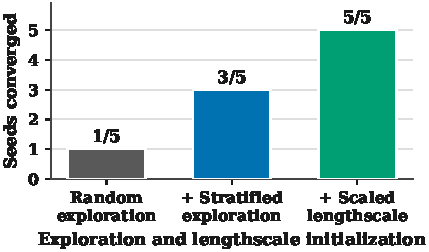
\includegraphics[width=\linewidth]{figs/fig_seed_reliability.pdf}
% \caption{Neither fix alone is sufficient: stratified exploration recovers
% 3/5 seeds and the scaled lengthscale is required to reach 5/5.}
% \label{fig:reliability}
% \end{figure}

% \subsection{Cross-Manipulator Evaluation}
% \label{sec:results-multiarm}

% The release-state search trains successfully on all four evaluated
% manipulators. Mean landing error ranges from 1.4 to 2.7~cm without
% per-arm policy tuning beyond the corresponding torque and velocity limits.
% This result indicates that the release-state formulation is not tied to the
% Gen3 geometry.

% \subsection{Learned Dynamics under Aerodynamic Drag}
% \label{sec:results-drag}

% We next vary payload drag from less than 1\% to approximately 19\% of
% gravity and compare the learned model against the analytical no-drag
% baseline. At low drag, the analytical model remains close to the observed
% optimum and model-based learning provides limited additional benefit. At
% higher drag, the analytical baseline reaches 4--6~cm error, whereas the
% learned model achieves 0.6--1.7~cm, corresponding to a 3--7-fold
% improvement.

% Object variation further shows constant landing error over payload masses
% of 30--150~g and diameters of 2--4.5~cm without retraining (all twelve
% mass/radius combinations fall within 1.38--1.46~cm), since drag stays small
% and the payload feedforward term directly accounts for the mass.

% \textbf{Interpretation.}
% The analytical baseline assumes drag-free ballistic motion, so its error
% grows with the object's aerodynamic drag; the learned GP instead fits the
% realized velocity change from data, so its accuracy does not depend on how
% large that drag term is. This is why the analytical model suffices at low
% drag and the learned model wins once drag becomes significant.

% This interpretation is qualitative rather than a fitted analytical model of
% the crossover. Determining the exact crossover point from a finer drag sweep
% remains future work.

% As an ablation, subtracting gravity as a GP mean function does not improve
% on the plain model here: error rises from 0.62 to 0.85~cm (Panda) and 1.69
% to 1.77~cm (KUKA), consistent with the mean function assuming the wrong
% dominant physics -- gravity, not drag -- in this regime.

% \subsection{Target-Height Generalization}
% \label{sec:results-height}

% A single policy trained on the KUKA iiwa over a continuous target-height
% range is evaluated on 100 fresh targets at heights not observed during
% training. It achieves 100\% successful throws, a mean landing error of
% 2.0~cm, and a worst-case error of 5.0~cm, with no systematic degradation
% over the evaluated height range (Fig.~\ref{fig:height-gen}).

% We also reproduce the zero-new-trials height-adaptation setting on the Gen3
% overhead configuration by reusing the trained GP and re-optimizing only the
% policy for three target heights.
% The resulting mean errors are 2.95, 3.41, and 3.80~cm for
% $h=0.10$, $0.20$, and $0.30$~m, respectively -- comparable to the 3.15~cm
% ground-level result and better than the 3.63~cm result from a complete
% 9-D retraining (Fig.~\ref{fig:height-adapt}).

% \begin{figure}[t]
% \centering
% 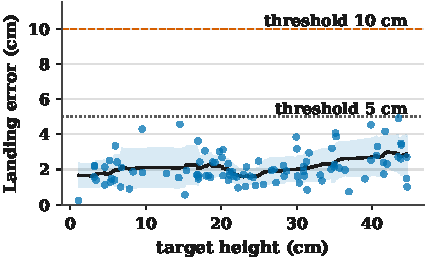
\includegraphics[width=\linewidth]{figs/fig_height_gen.pdf}
% \caption{Landing error stays well under both thresholds across the full
% height range on the KUKA iiwa, with no upward trend near either edge.}
% \label{fig:height-gen}
% \end{figure}

% \begin{figure}[t]
% \centering
% 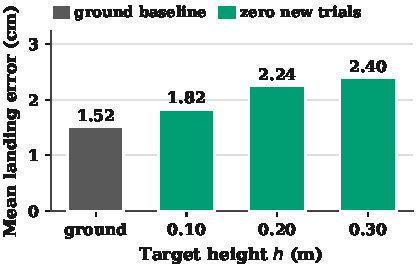
\includegraphics[width=\linewidth]{figs/fig_height_adaptation.pdf}
% \caption{Adapting to a new target height costs zero additional robot trials
% and still beats a full 9-D retrain (3.63~cm) at every height tested.}
% \label{fig:height-adapt}
% \end{figure}

% \subsection{Low-Torque Throwing and Feasible Range}
% \label{sec:results-overhead}
% For the Gen3, the fixed low-release posture does not provide a useful
% high-elevation throw. Increasing elevation under that posture decreases the
% achievable range, causing distance optimization to favor a near-horizontal
% motion. In contrast, searching over the release state under the complete
% feasibility cascade identifies a genuine overhead throwing configuration.

% The selected configuration reaches a release height of approximately
% 1.1~m. When windup, release, and post-release recovery constraints are all
% enforced, the maximum simulated safe-throw distance is 0.82~m, compared with
% the arm's 0.87~m kinematic reach under the considered setup
% (Fig.~\ref{fig:range-ceiling}). This value is best interpreted as a measured
% capability boundary of the simulated low-torque platform rather than as an
% extended-reach result.

% For this configuration, the mean landing error is 3.15~cm over 30 unseen
% targets, with 100\% of throws within 10~cm. The release speed varies from
% 1.16 to 1.49~m/s over the target-distance range rather than saturating at a
% single maximum value.

% \begin{figure}[t]
% \centering
% 
\includegraphics[width=0.9\linewidth]{results/final_figures/fig_range_ceiling.png}
% \caption{Simulated safe-throw range boundary of 0.82~m compared with the
% 0.87~m kinematic reach of the Kinova Gen3 under the considered constraints.}
% \label{fig:range-ceiling}
% \end{figure}

% \subsection{Impact of Whole-Trajectory Feasibility}
% \label{sec:results-ablation}

% We quantify the effect of whole-trajectory feasibility by applying the same
% release-pose and direction enumeration to the Gen3 and Franka Panda. For
% each candidate that passes the release-instant criterion, we record whether
% it also satisfies the complete feasibility cascade
% (Table~\ref{tab:ablation}).

% \begin{table}[t]
% \centering
% \small
% \caption{Release-instant-only versus whole-trajectory feasibility for the
% Gen3 and Franka Panda using the same posture and direction grid.}
% \label{tab:ablation}
% \begin{tabular}{@{}lcc@{}}
% \toprule
%  & Gen3 & Panda \\
% \midrule
% Release-instant-feasible & 446{,}071 & 152{,}844 \\
% Also full-traj.-feasible & 74{,}230 (16.6\%) & 152{,}844 (100\%) \\
% Rej.\ windup-path & 242{,}725 (54.4\%) & 0 \\
% Rej.\ throw-ramp & 66{,}706 (15.0\%) & 0 \\
% Rej.\ follow-through & 62{,}410 (14.0\%) & 0 \\
% Best range, instant-only & 1.03 m & 1.65 m \\
% Best range, full check & 0.82 m & 1.65 m \\
% \bottomrule
% \end{tabular}
% \end{table}

% For the Gen3, the complete cascade rejects 83.4\% of candidates that would
% have been accepted by the release-instant-only criterion. The largest source
% of rejection is the windup-path check, which accounts for 54.4\% of the
% release-instant-feasible candidates in the reported cascade order. The
% throw-ramp and follow-through stages account for 15.0\% and 14.0\%,
% respectively.

% The resulting best range decreases from 1.03~m under the release-instant
% criterion to 0.82~m after whole-trajectory validation, corresponding to a
% 20\% reduction. This difference demonstrates that release-state feasibility
% alone can overestimate the motion that the manipulator can execute and
% recover from.

% For the Panda, none of the 152{,}844 release-instant-feasible candidates is
% rejected by the full cascade, and the best candidate remains 1.65~m under
% both criteria.

% \textbf{Isolating torque headroom as the causal variable.} The Gen3/Panda
% contrast above differs in both torque budget and kinematics simultaneously,
% so it cannot by itself distinguish whether whole-trajectory rejection is
% driven by torque headroom or is specific to the Gen3's geometry. To isolate
% torque as the sole independent variable, we re-ran the same candidate
% enumeration and feasibility cascade on six synthetic profiles that are
% bit-for-bit copies of the Gen3 (identical URDF, $q_{\mathrm{neutral}}$,
% $\dot q^{\max}$, and control gains) with only $\tau_{\max}$ scaled by a
% factor $k$ relative to the real Gen3's 39/9~Nm limits
% (Fig.~\ref{fig:torque-sweep}, Table~\ref{tab:torque-sweep}).

% \begin{figure}[t]
% \centering
% 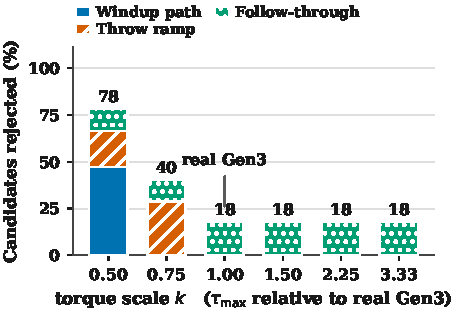
\includegraphics[width=\linewidth]{figs/fig_torque_sweep.pdf}
% \caption{Rejection falls monotonically with torque headroom under fixed
% kinematics, and the dominant failure stage shifts as it does: the windup
% path saturates the budget at low torque, the throw ramp takes over, and
% follow-through remains an irreducible floor that added torque cannot
% remove. Rates are shares of the release-instant-feasible pool, which is
% itself torque-dependent (Table~\ref{tab:torque-sweep}).}
% \label{fig:torque-sweep}
% \end{figure}

% \begin{table}[t]
% \centering
% \small
% \caption{Torque-headroom sweep on Gen3-identical kinematics. The
% release-instant-feasible pool shrinks with $\tau_{\max}$ as well, so the
% rejection rates in Fig.~\ref{fig:torque-sweep} are taken over a
% torque-dependent denominator.}
% \label{tab:torque-sweep}
% \begin{tabular}{@{}lrrrr@{}}
% \toprule
% $k$ & wrist $\tau_{\max}$ & instant- & full-traj- & rej. \\
%     & (Nm)                & feasible & feasible   & (\%) \\
% \midrule
% 0.50 & 4.5   & 118{,}954 & 0         & 100.0 \\
% 0.75 & 6.75  & 344{,}477 & 0         & 100.0 \\
% 1.00\rlap{$^{\dagger}$} & 9.0 & 446{,}071 & 74{,}230  & 83.4 \\
% 1.50 & 13.5  & 475{,}123 & 261{,}945 & 44.9 \\
% 2.25 & 20.25 & 475{,}123 & 391{,}238 & 17.7 \\
% 3.33\rlap{$^{\ddagger}$} & 29.97 & 475{,}123 & 391{,}238 & 17.7 \\
% \bottomrule
% \end{tabular}

% \vspace{2pt}
% {\footnotesize $^{\dagger}$reproduces the real Gen3 bit-identically.
% $^{\ddagger}$approximates the Panda's torque \emph{ratio} only, not its
% kinematics.}
% \end{table}

% Rejection falls monotonically with torque headroom while kinematics,
% joint-limit structure, and control gains are held fixed across every row,
% demonstrating that torque headroom is causal rather than an artifact of
% comparing two different arms. Two further properties are visible. Below
% $k\approx0.75$, no candidate survives the full cascade: the effect is total
% infeasibility, not merely reduced range. Rejection also saturates at
% 17.7\% rather than reaching 0\% -- windup-path and throw-ramp failures
% vanish with added torque, but follow-through failures do not, leaving a
% residual floor driven by the Gen3's own kinematics. That floor is why the
% sweep never reaches the Panda's real 0\%, whose kinematics it does not
% reproduce, and it shows the cascade catching two distinct failure
% mechanisms, torque-driven and kinematics-driven, that a torque-only
% analysis would miss.

% \subsection{Computational Efficiency}
% \label{sec:results-cost}

% A complete Gen3 overhead-throw training run (10 trials, five exploration,
% $N_{\mathrm{opt}}=1500$ policy-optimization steps per trial, reusing a
% precomputed release-pose table) takes 17~min~44~s on a single CPU core,
% 1.11~GB peak memory. The one-time release-state search
% ($\sim\!9\times10^4$ posture candidates before pruning) takes 28~min~27~s on
% the same machine. Both costs are incurred once per arm/workspace geometry;
% the pose table is then reused across all training seeds and evaluation
% targets.

% \subsection{Hardware Validation}
% \label{sec:results-hw}

% The real Kinova Gen3 is used to validate the unloaded components of
% the execution pipeline. State read-back, gripper actuation, full-speed
% joint-velocity streaming, gripper-latency compensation, and the open-loop
% drift budget have been validated on the physical arm
% (Table~\ref{tab:hw-status}).

% During bring-up, five hardware-specific effects were identified. Joint
% angles are reported over a $[0^\circ,360^\circ)$ convention, requiring
% different handling for continuous and limited joints. Gripper-open latency
% was measured as $67.9\pm6.4$~ms from 1~kHz UDP feedback. At the
% 1.498~m/s release speed considered in the overhead configuration, an
% uncompensated delay would correspond to approximately 10.2~cm of travel.
% The executor therefore applies a wall-clock lead-time compensation.

% The joint-speed streaming interface has a measured ceiling of 40~Hz.
% Open-loop position drift during the throw was measured as 0.0171~rad at
% release, corresponding to approximately 1.0~cm of landing error under the
% reported conversion. A remaining implementation-level contribution is the
% 25~ms command interval, corresponding to approximately 3.7~cm at the
% considered release speed (Fig.~\ref{fig:error-budget}).

% \begin{table}[t]
% \centering
% \small
% \caption{Real Kinova Gen3 hardware bring-up status.}
% \label{tab:hw-status}
% \begin{tabular}{@{}p{4.6cm}c@{}}
% \toprule
% Stage & Status \\
% \midrule
% Read-only state (joints, gripper) & live \\
% Gripper actuation & live \\
% Full-speed joint-velocity streaming & live \\
% Gripper latency compensation & done \\
% Open-loop drift budget & in budget \\
% Loaded throw (ball in gripper) & pending \\
% Real landing measurement & pending \\
% \bottomrule
% \end{tabular}
% \end{table}

% \begin{figure}[t]
% \centering
% 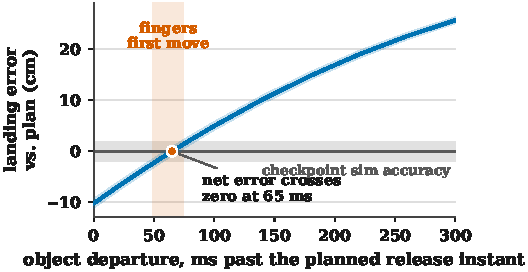
\includegraphics[width=\linewidth]{figs/fig_error_budget.pdf}
% \caption{Uncompensated gripper latency would dominate the sim-to-real error
% budget at 3.5$\times$ the simulation accuracy itself (dashed line), which is
% why it is compensated in the executor. Quantities are measured
% independently and do not constitute a combined real throwing result.}
% \label{fig:error-budget}
% \end{figure}

% At the current stage, the hardware validation therefore establishes the
% operation of the execution stack but does not establish physical throwing
% accuracy. In particular, the planned release speed is approximately
% 1.498~m/s, while the applicability of the documented 0.500~m/s Cartesian
% speed ceiling to joint-speed streaming mode has not yet been established.
% Consequently, no real landing result is reported.

% \section{Discussion}

% The experiments support three main conclusions. First, the release
% configuration should not necessarily be treated as a fixed design parameter
% when transferring model-based throwing to manipulators with different
% actuator capabilities. Explicitly searching the release state allows the
% throwing policy to operate within the available torque and velocity
% envelope. Second, feasibility must be
% considered over the complete motion: for the Gen3, release-instant
% feasibility alone accepts a large fraction of candidates that later violate
% trajectory constraints. Third, model-based learning is most beneficial when the analytical dynamics
% become inaccurate, as demonstrated by the observed drag-regime crossover.

% \textbf{Limitations.} Five factors should be considered when interpreting these results.
% First, the throwing-accuracy results are simulation-based. Although the
% unloaded-stage hardware pipeline has been validated on the Gen3, a loaded
% physical throw and corresponding landing measurement are not yet available.
% Second, the Gen3 implementation currently treats gripper delay as a measured
% point estimate with fixed lead-time compensation, rather than learning a
% distribution of release delays as in the original MC-PILOT formulation.
% Third, object and multi-manipulator generalization are evaluated in
% simulation; the real hardware study is currently limited to the Gen3.
% The multi-manipulator controllers also share a single computed-torque gain
% set across arms with different link masses; per-arm tracking accuracy has
% not been independently verified.
% Fourth, a gripper-offset-corrected training run also exists for the Gen3 overhead
% configuration (Sec.~\ref{sec:method-torque}) but converges to a different
% release geometry ($15^\circ$ elevation, 2.07~m/s) than
% Secs.~\ref{sec:results-overhead}--\ref{sec:results-ablation} analyze;
% reconciling the two is left for future work.
% Finally, the release-state search is a discrete enumeration followed by
% per-candidate feasibility evaluation. It is intentionally simpler than a
% general continuous trajectory optimizer, but its computational cost depends
% on the resolution of the candidate grid.

% The reported reliability analysis also highlights the importance of
% multi-seed evaluation in model-based policy search. A single successful
% optimization run can provide an incomplete picture of convergence
% reliability. We therefore use multiple seeds and evaluate final policies on
% fresh targets rather than relying on training-time particle cost.

% For reproducibility, the release-state search solver, feasibility checker,
% multi-manipulator evaluation scripts, and trained GP/policy checkpoints for
% the simulation experiments will be released publicly upon publication,
% together with a regression suite that encodes each previously found
% planning or control defect as a test.

% \section{Conclusion}

% We presented a constraint-aware extension of model-based robotic
% pick-and-throw in which the release state is selected according to the
% manipulator's kinematic and dynamic capabilities rather than fixed a priori.
% The approach combines release-state search with Gaussian-process dynamics
% learning and particle-based policy optimization, while evaluating torque and
% velocity feasibility over the complete windup, throw, and follow-through
% motion.

% Across four simulated manipulators, the resulting framework achieves
% 1.4--2.7~cm mean landing error without per-arm policy tuning beyond the
% corresponding actuator limits. On the Kinova Gen3, whole-trajectory
% feasibility identifies a 0.82~m safe-throw boundary under the considered
% configuration and constraints. Additional experiments demonstrate
% continuous target-height generalization and show that model-based learning
% provides its largest benefit when aerodynamic drag makes a no-drag
% analytical model inaccurate.

% The physical Gen3 experiments currently validate the unloaded stages of the
% execution pipeline, including state feedback, gripper actuation, velocity
% streaming, and latency compensation. Physical throwing and landing
% measurements remain to be completed. Thus, the present results establish the
% simulation-side effectiveness and the hardware execution readiness of the
% proposed constraint-aware formulation, while leaving full real-world
% throwing evaluation as the next experimental step.


% %%%%%%%%%%%%%%%%%%%%%%%%%%%%%%%%%%%%%%%%%%
% \bibliographystyle{ieeetr}
% \bibliography{reference}

% \end{document}
